\documentclass{extarticle}

% Para la fuente y el interlineado
%\usepackage{fontspec}
%\setmainfont{Arial}
\renewcommand{\baselinestretch}{1.5}

% para poder escribir con tildes
\usepackage[T1]{fontenc}
\usepackage[utf8]{inputenc}
\usepackage[spanish]{babel}

\usepackage{listings}
\usepackage{amsmath}
\usepackage{amsfonts}
\usepackage[margin=1.3in]{geometry}
\usepackage{graphicx}
\usepackage[colorinlistoftodos]{todonotes}
\usepackage{hyperref}
\newcommand{\squeezeup}{\vspace{-5.0mm}}

% Para el header y el footer
\usepackage{fancyhdr}
\pagestyle{fancy}
\fancyhf{}
\rhead{MOR}
\lhead{Germán Faller  \& Octavio Perez Kempner}
\rfoot{\thepage}

% Datos de autor
\title{Metaheurísticas y Optimización Sobre Redes - Obligatorio 2017}
\author{Germán Faller y Octavio Perez Kempner}
\date{v1.0}


\begin{document}

\begin{titlepage}
    \begin{center}
    	
\includegraphics[width=2cm]{img/logo_FING_rgb.jpg}
    	\\
        \vspace*{1cm}
        \huge{\textbf{Metaheurísticas y Optimización Sobre Redes}}
        
        \vspace{0.5cm}
       Obligatorio 2017
        \vspace{2cm}
        \vfill
        \Large{
        Germán Faller \& Octavio Perez Kempner\\Docente: Dr. Ing. Claudio Risso \\ Instituto de Computación \\ Facultad de Ingeniería}
        
        \vfill
        \vspace{0.8cm}
    \end{center} 
\end{titlepage}

\tableofcontents 

\newpage
\section{Introduccion}

El obligatorio a resolver consiste en abordar el problema de diseñar una red de Trenes Ligeros (Light Rail Transit o LRT) para Montevideo.

Considerando como característico de nuestra capital el tener una población que tiende a vivir lejos de su centro de estudio y/o trabajo, se supondrá que en la ciudad existen tres puntos de concentración: Tres Cruces, Palacio Municipal y la Plaza Independencia que serán los destinos de los pasajeros en la mañana y su punto de partida en la tarde. Se asumirá que se contará con la infraestructura adecuada para que al llegar a cualquiera de estos puntos la movilidad urbana entre ellos será rápida.

Por otra parte identificamos cuatro agregadores zonales, las terminales: Cerro, Colón, Carrasco y Pocitos. Se tendrá como objetivo de la red definir los caminos desde cualquier agregador zonal a cualquier punto de concentración.

A continuación se muestran las terminales, los puntos de concentración y los tramos posibiles a seleccionar para construir la red LRT.
\begin{align*}
	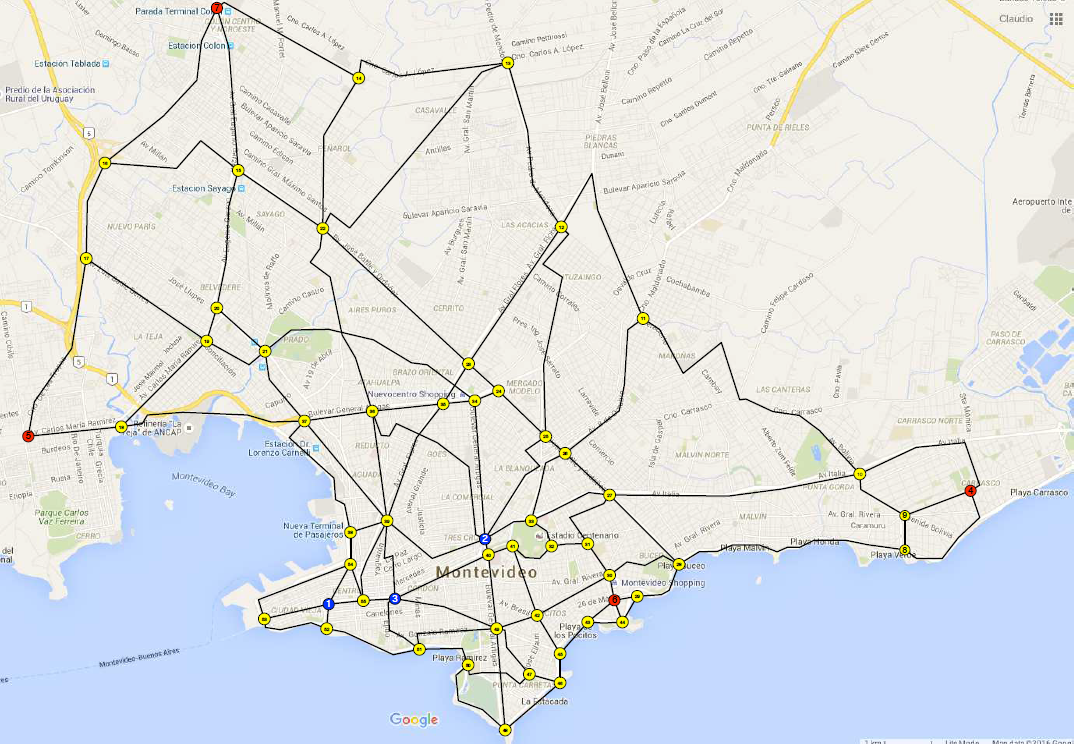
\includegraphics[scale=0.7]{img/FullMap.png}
\end{align*}

En las siguientes secciones se presentarán los distintos desafíos del obligatorio y conjuntamente con las soluciones propuestas.


\newpage
\section{Parte I - Primera aproximación}
\subsection{Minimización por costos}
En una primera aproximación el objetivo fue obtener el trazado de costo mínimo para conectar las terminales con los puntos de concentración planteando el problema como uno de programación lineal (LP) y considerando las siguientes restricciones:
\begin{itemize}
	\item Que existan dos líneas (caminos) para conectar tanto Cerro, Colón y Carrasco con los nodos del centro y tres líneas para conectar Pocitos con los nodos del centro.
	\item Que ninguno de los tramos del plano fuera utilizado por más de una línea (las estaciones sí pueden ser parte de más de una línea).
\end{itemize}

\subsubsection*{Formulación LP}
	min $\sum_{(i,j) \in E} c_{ij}.x_{ij}$\
    
	s.t. 
    
	$\sum_{j \in S(i)} x_{ij} - \sum_{j \in E(i)} x_{ji} =
	\bigg\{ \begin{matrix} 
        0 &\text{ si i es un nodo interno del camino}  \\
        f_{i} &\text{ (flujo saliente de i), si i es una terminal}
      \end{matrix}$\\
      
    $ 0  \leq x_{ij}  \leq  1$\

Considerando entonces el costo total mínimo, se obtuvo que este era de 18076, a continuación se muestra la solución obtenida:
\begin{align*}
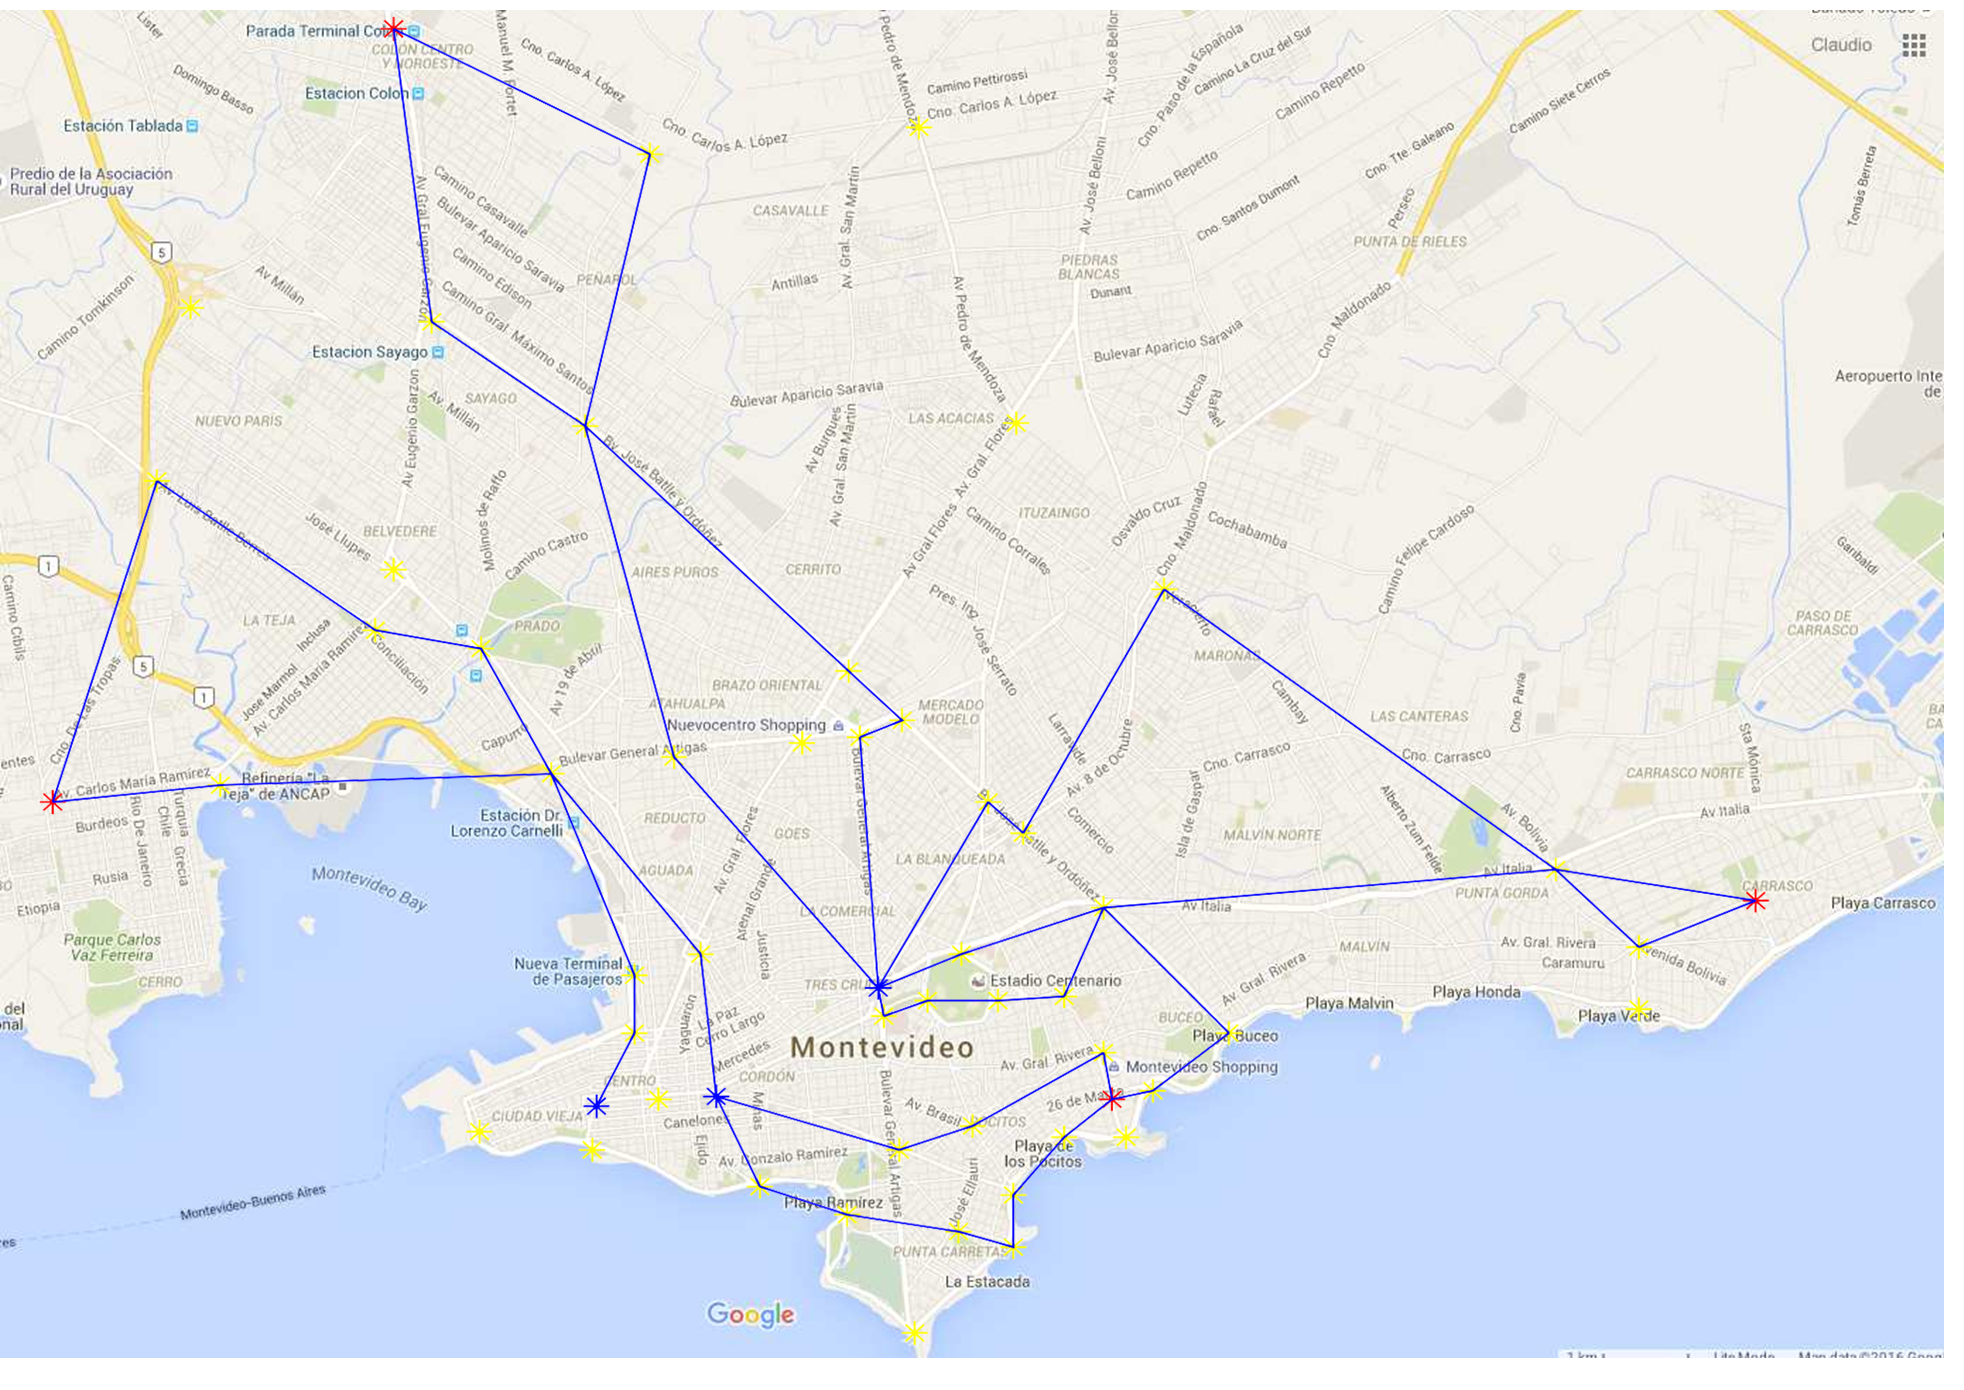
\includegraphics[scale=0.3]{img/f1.png}
\end{align*}
\newpage
\subsection{Minimización por delay}
Una variante del problema anterior a resolver es la minimización por delay en lugar de costos que resulta análoga a la anterior (considerando la columna de delay en lugar a la de costos).

En este caso el óptimo hallado se corresponde a un delay total de 8512, a continuación se muestra la solución obtenida:
\begin{align*}
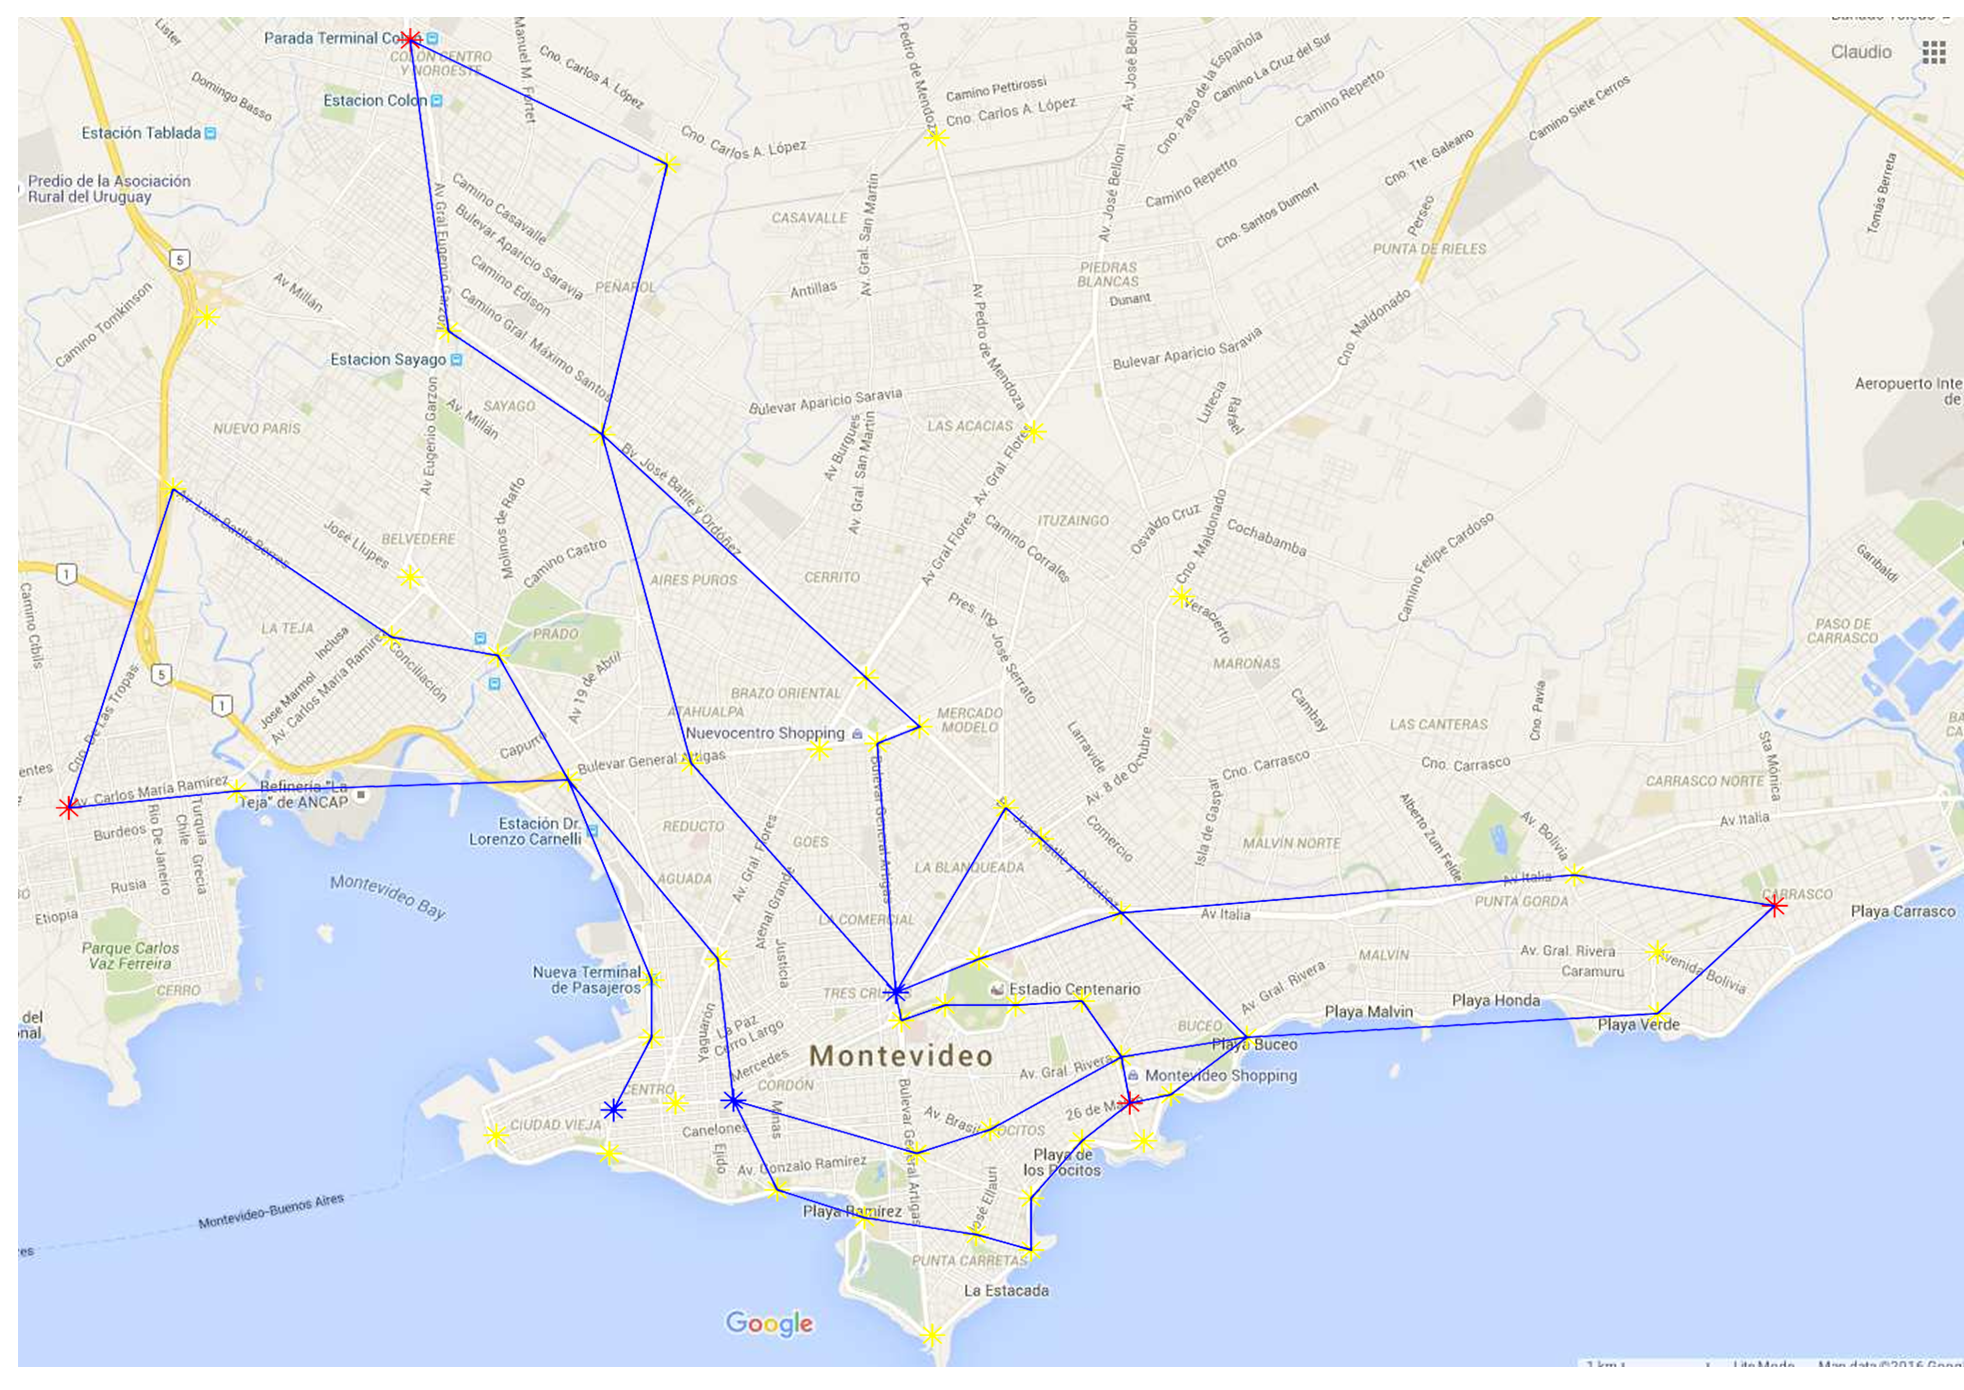
\includegraphics[scale=0.3]{img/f2.png}
\end{align*}

\subsection{Caminos de costo mínimo}
Como última variante en esta primera parte se calcularon los caminos de costo mínimo, el total fue de 7257, la solución obtenida se muestra a continuación:
\begin{align*}
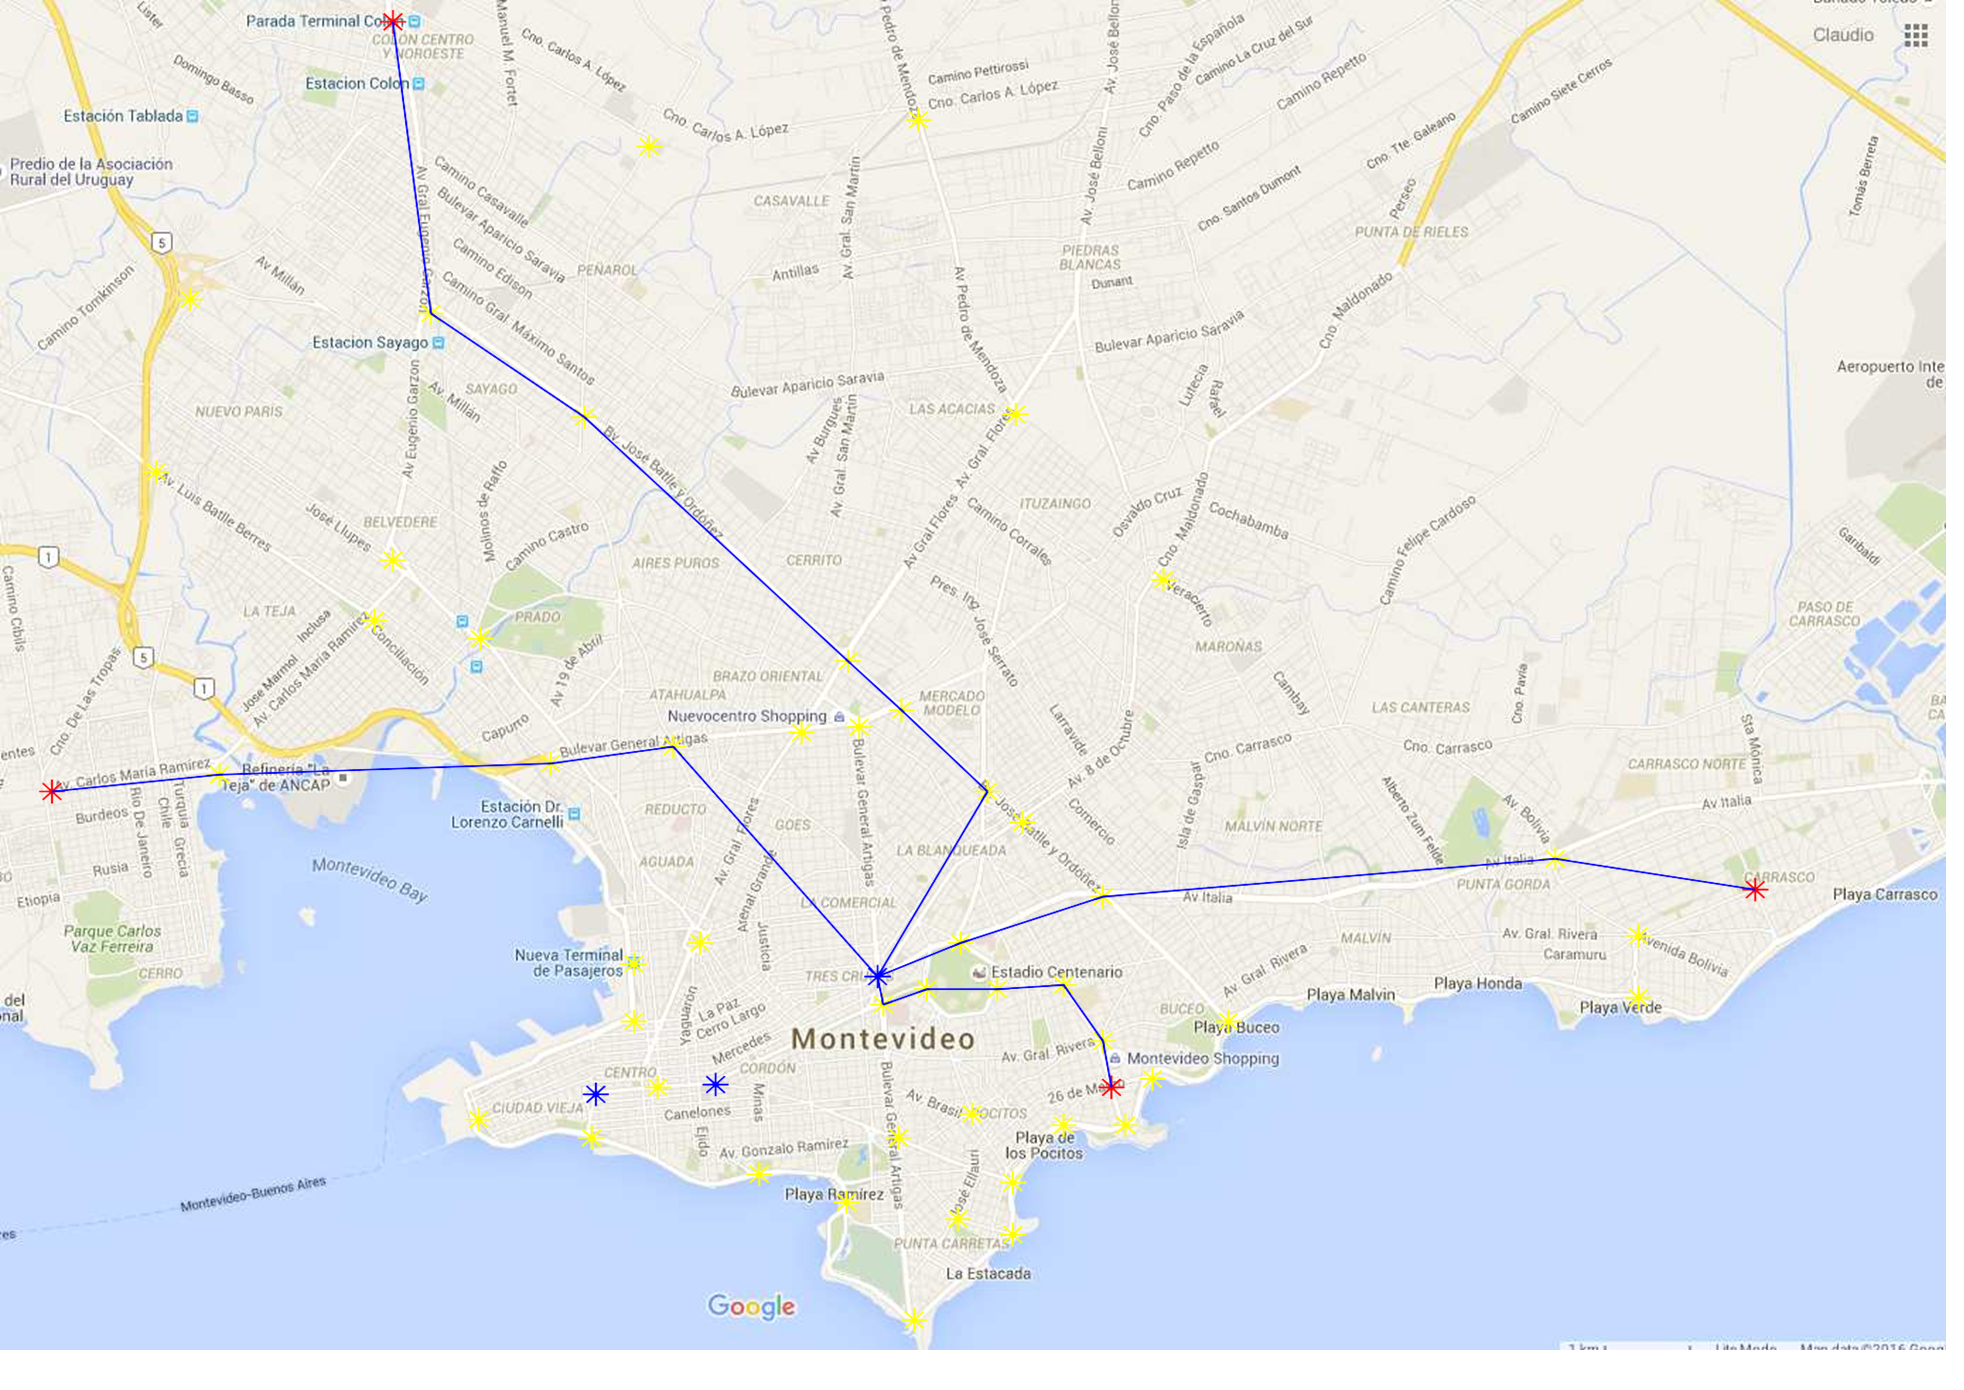
\includegraphics[scale=0.3]{img/f3.png}
\end{align*}
\subsection{Comparación de resultados}
La siguiente tabla consolida las distintas propuestas considerando para cada una el mínimo total y sus respectivos valores en costo/delay.

\begin{table}[h!]
	\centering
	\caption{Resultados}
	\label{table:levels-sequence}
	\begin{tabular}{|l|l|l|} \hline
		Objetivo  &   Costo Total    & Delay Total   \\
		\hline
		Total por costos        &  118076    & 8700  \\  
		\hline
		Total por delay     &  182572 & 8512 \\
		\hline
		Único camino por costos  &  7257  & 3513  \\
		\hline
		Único camino por delay    &  7850    & 3229   \\
		\hline
	\end{tabular}
\end{table}

Cabe notar que en cualquier caso la complejidad del problema es polinomial dado que cuando tenemos múltiples fuentes y sumideros estos problemas se pueden resolver con el algoritmo de Ford-Fulkerson mientras que en el caso de tener caminos únicos alcanza con el algoritmo de Dijkstra que es también de orden polinomial.

\section{Parte II - Reutilización de tramos}
Bajo las mismas condiciones que la parte anterior se busca ahora la reutilización de tramos entre líneas de distinto origen. Esta nueva versión es una relajación del problema anterior dado que soluciones del problema anterior ademas son soluciones en esta nueva versión.
Naturalmente, dado que el objetivo continúa siendo la minimización de costos, al poder reutilizar tramos entre líneas de distinto origen, el mínimo encontrado conecta los agregadores y algunos de ellos al centro, por lo que el delay se ve sensiblemente afectado respecto a la solución de la versión anterior.

\subsection{Formulación MIP}
    
	min $\sum_{(i,j) \in E} c_{ij}.u_{ij}$\
    
	s.t. 
    
	$\sum_{j \in S(i)} x^k_{ij} - \sum_{j \in E(i)} x^k_{ji} =
	\bigg\{ \begin{matrix} 
        0 & \text{  } \forall i \not = k &\text{  (equilibrio de flujo)}  \\
        f_{i} & \text{  } \forall i = k &\text{  (flujo saliente de la fuente)}
      \end{matrix}$\
      
    $ 0  \leq  x^k_{ij}\leq u_{ij} \leq  1$, $ \forall k \in \{4,5,6,7\}$

\subsection{Resultados}
El costo de construir estos caminos fue de 9109 y la imagen correspondiente a la solución óptima obtenida se encuentra a continuación:
\begin{align*}
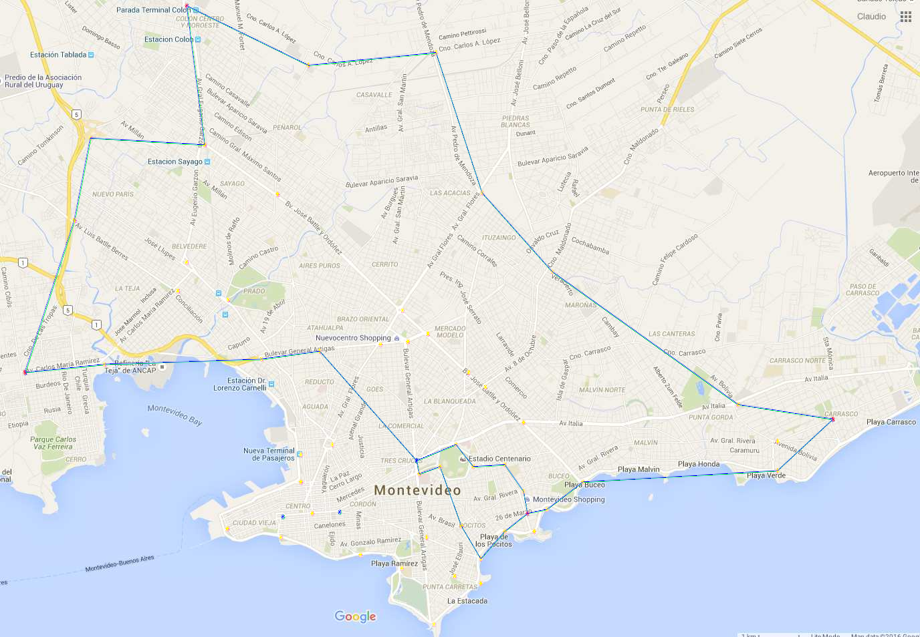
\includegraphics[scale=0.6]{img/g1.png}
\end{align*}

\begin{table}[h!]
	\centering
	\caption{Delay por tramos}
	\label{table:delay-tramos}
	\begin{tabular}{|l|l|l|l|l|} \hline
		Concentrador  &   Total P1    & Promedio P1 & Total P2    & Promedio P2   \\
		\hline
		Carrasco        &  2131 & 1066 & 4804 & 2402  \\  
		\hline
		Cerro     &  2045 & 1023 & 4804 & 2402  \\
		\hline
		Pocitos  &  2063 & 688 &  5453 & 1818 \\
		\hline
		Colon    &  2192 & 1096 &  4804 & 2402   \\
		\hline
	\end{tabular}
\end{table}
En esta tabla puede apreciarse el aumento del delay al reutilizar al máximo los tramos. Este problema motiva la búsqueda de variantes en la siguiente sección para lograr costos razonables sin comprometer los delays de la red más allá de algún umbral establecido.

%Esto de abajo es una tabla que no va aparecer en el Documento
\iffalse

car 4 8 28 29 6            		-> 202 322 132 91 = 747
car 4 10 11 12 13 14 7			-> 248+ 419+ 300+ 257+ 249+244=1717
cer 5 17 16 15 7				-> 274+ 174+ 236+ 245=929
cer 5 18 37 36 2				-> 168+ 272+ 141+ 296=877
poc 6 29 28 8 4					-> 202+ 322+ 132+ 91=747
poc 6 30 31 32 33 2				-> 94+ 108+ 106+ 104+ 122 =534  *
poc 6 43 45 42 41 40 2			-> 104+ 112+ 115+ 146+ 94+ 78=649
col 7 14 13 12 11 10 4			-> 248+ 419+ 300+ 257+ 249+ 244=1717
col 7 15 16 17 5				-> 274+ 174+ 236+ 245=929

4 6 2		-> 747+534=1281
4 7 5 2		-> 1717+929+877=3523

6 2			-> 534
6 2			-> 649
6 4 7 5 2	-> 747 + 1717+929+877=4270

7 4 6 2		-> 1717+747+534=2998
7 5 2		-> 929+877=1806

5 2			-> 877
5 7 4 6 2	-> 929+ 1717+747+534=3927
\fi


\newpage
\section{Parte III - Algunas variantes}
El KnapSack Problem (KSP) puede verse como un problema de optimización en el que se busca maximizar la ganancia de artículos incluídos en la mochila considerando que los pesos respectivos de los objetos no superen un umbral total. La siguiente es una formulación LP de este problema:
\begin{equation}
\begin{array}{rrclcl}
\displaystyle \max & \sum_{i=0}^{n} v_ix_i  \\
\textrm{s.t.} & \sum_{i=0}^{n} p_ix_i & \leq & b \\
& 0 \geq x_i & \geq & 1  &, & \forall i \in N \\
\end{array}
\end{equation}

Por otra parte, el problema del camino de costo mínimo (CCM) consiste en encontrar un CCM dados dos vértices s y t en un grafo G. En este problema el costo está dado por el peso de la arista pero existen varias variantes a este problema que incluyen restricciones adicionales dando lugar a una familia de problemas que recibe el nombre de Constrained Shortest Path Problems (CSPP).

Si suponemos que las aristas tienen dos atributos diferentes (peso y costo) y que queremos encontrar el CCM restricto a que los pesos de las aristas del camino no superen un umbral dado tenemos una variante del CCM que resulta ser la instancia más sencilla del problema a resolver en esta parte dado que como mínimo siempre tendremos al menos una fuente y un sumidero.

Por lo tanto, si probamos que esta variante es NP-C el problema de esta parte también será NP-C dado que en todas sus instancias precisaremos resolver al menos una vez un problema que es NP-C.
Cabe notar que al probar la NP-Completitud del problema queda demostrado que este es NP-Hard por definición de NP-Completitud.

Realizaremos la prueba a partir de una reducción del KSP a la variante del CCM descrita anteriormente.

\newtheorem{demo}{\scshape{Demostración}}
\begin{demo}
	Dada una instancia del KnapSack con artículos en \{1,...,n\}, cada uno de valor $v_{i}$ y peso $p_{i}$, para cada $j=1,...,n$, construiremos un grafo de $n$ nodos de la siguiente forma:
	\begin{align*}
	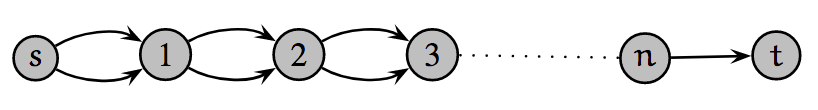
\includegraphics[scale=0.7]{img/grafoDemo}
	\end{align*}
	
	En este grafo de aristas paralelas asociaremos a las superiores las tuplas $(M-v_{j},p_{j})$\footnote{$M = max\{v_{j}: j=1,..,n-1\}$} y $(M,0)$ a las inferiores considerando que en la variante del CCM el costo se corresponde con el primer componente de una tupla y la cantidad máxima de flujo de una arista con la segunda componente.
	
	Luego, podemos ver entonces que si existe un camino de costo mínimo en el grafo que cumpla con las restricciones de flujo encontramos una solución para el KSP y viceversa con lo cual hemos encontrado una reducción y por tanto que la variante de esta parte es un problema NP-C.
		
\end{demo}	

\section{Parte IV - Abordaje por Metaheurísticas}
\subsection{Introducción}
La metaheurística escogida para atacar el problema de esta parte ha sido Computación Evolutiva. Dentro de este espectro de técnicas se ha optado en particular por implementar un algoritmo genético con operadores de cruzamiento y mutación.

Como principales motivos de la elección se destacan los siguientes:
\begin{itemize}
	\item La representación de individuos resulta bastante directa al considerar como genes de un individuo a los caminos que conforman una solución del problema.
	\squeezeup
	\begin{center}
		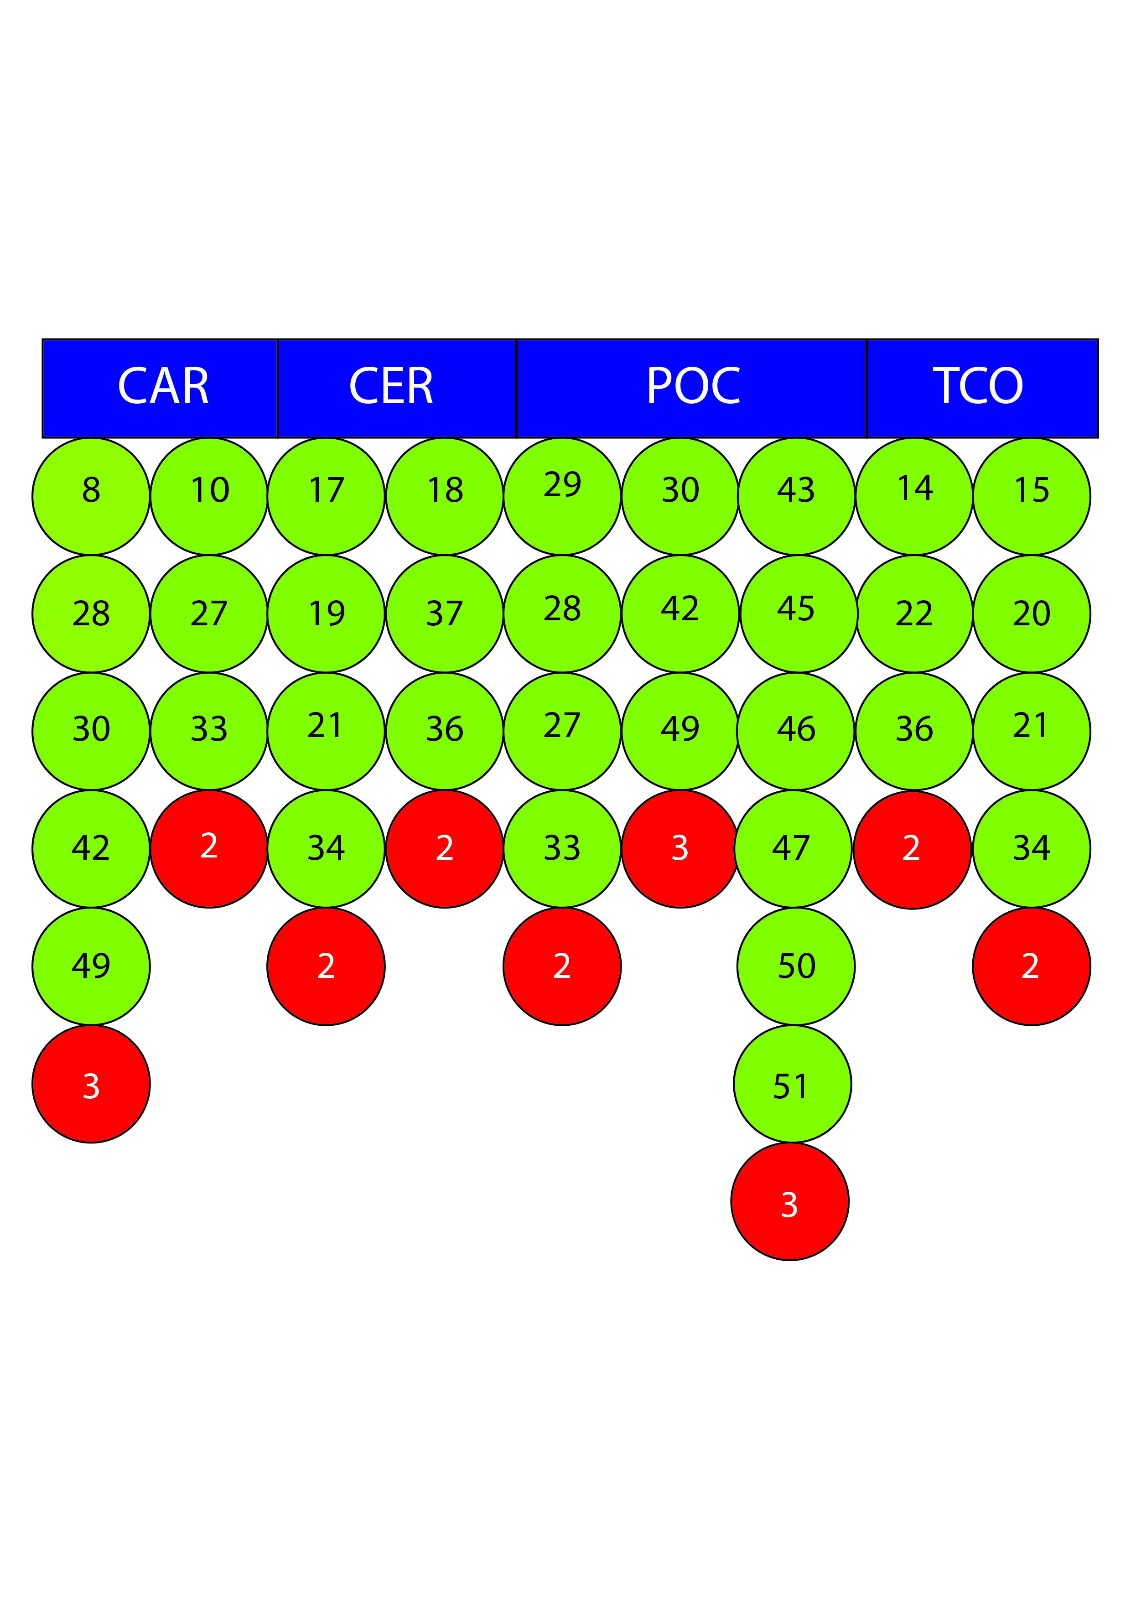
\includegraphics[scale=0.1]{img/genindividuo.jpeg}
	\end{center}
	\squeezeup
	\item La función de fitness para evaluar a los individuos resulta sencilla como expresión del costo.
	\item La generación de una población inicial para este tipo de problemas puede hacerse polinómicamente y con un muestreo considerable resolviendo independientemente cada subproblema del grafo y combinando soluciones.
	\item Los operadores de cruzamiento y mutación también tienen una traducción casi directa en términos de caminos y genes de los individuos.
	\item La exploración del espacio de búsqueda también resulta natural a partir de la variedad de la población inicial y las posibilidades que surgen de la aplicación de los operadores.
\end{itemize}

En definitiva, al momento de optar por esta metaheurística se valoró la sencillez de la tradución de este problema en particular de grafos a uno de algoritmos genéticos, que la función de fitness no insumiera un overhead considerable (evaluar a un individuo) y que los parámetros de ajuste tendieran a ser pocos a partir de aprovechar una variedad inicial dada por la aleatorización de los caminos iniciales para cada individuo.


\subsection{Inicialización}
En esta sección se desarrollan las ideas que se llevaron a cabo para obtener una población inicial mostrando la factibilidad de las propuestas elaboradas. Los resultados de las pruebas realizadas se documentan en el Anexo I mientras que el resto de los detalles se encuentran en el Anexo II.

En primer lugar se observó que la solución de la parte I constituye un individuo factible para esta parte por lo que la misma (considerada como individuo) fue agregada a la población inicial.

En segundo lugar, se tomó la decisión de perturbar los costos en el grafo original para buscar nuevas soluciones que pudieran generar individuos factibles. Para esto el procedimiento fue el siguiente:
\begin{itemize}
	\item Se redujo el problema de la parte I a una única fuente manteniendo todos los sumideros. Esto se hizo para cada fuente.
	\item Luego, sobre instancias del grafo original perturbado se fueron resolviendo los subproblemas descritos anteriormente de manera independiente.
	\item A partir de lo anterior se obtuvieron soluciones perturbadas y parciales de las distintas fuentes a los sumideros.
	\item Sobre las soluciones parciales factibles en el grafo original (considerando esta vez la cota de delay de las mismas) obtenidas de esta forma, se obtuvieron soluciones completas a partir de combinar unas con otras.
\end{itemize}

Cabe destacar que como las soluciones parciales respondían a subproblemas de la parte I (al considerar una única fuente) su cálculo resultó sencillo y a la vez al calcular cada una sobre una instancia independiente del grafo original perturbado y con todas las aristas, al combinarlas para generar un individuo se permitía que se compartieran caminos entre líneas de terminales distintas.
Por otra parte, al seguir este enfoque si uno considera al menos una solución parcial con su contraparte de la parte I se tienen al menos dos opciones posibles como líneas para una fuente a los sumideros por lo que realizando todas las combinaciones posibles se obtienen unos 16 individuos.

Experimentalmente, perturbando el grafo original en un rango 0-50\% se observó que:
\begin{itemize}
	\item Al menos el 50\% de las soluciones parciales obtenidas eran factibles en el grafo original.
	\item Dentro de las soluciones parciales factibles obtenidas se encontraron: 2 para TCO, 3 para CRO, 2 para POC y 4 para CAR.
\end{itemize}

\subsection{Selección}
La selección para dar lugar a una nueva generación será basa en ranking. Todos los individuos serán rankeados y su probabilidad a ser seleccionados para el cruzamiento será inversamente proporcional a su valor en dicho ranking (a menor costo total mayor probabilidad de reproducción).
Una vez seleccionados dos individuos el producto de su cruzamiento será agregado a la población actual y recién en dicho momento se descartará al miembro más débil. Así con cada iteración.

Considerando que este método puede resultar elitista e ir en detrimento de la diversidad, se estudiará la idea de parametrizar la selección permitiendo que cada cierto tiempo y con una probabilidad a definir, uno de los individuos a reproducirse sea tomado de los últimos lugares del ranking (con peor costo).

\subsection{Cruzamiento y mutaciones}
\begin{itemize}
	\item (Cruzamiento) El principal operador de cruzamiento será la selección de líneas correspondientes a una fuente dada. Es decir que considerando padre y madre, el hijo de ambos resultará de seleccionar equiprobablemente las líneas de una fuente para cada fuente (el hijo o bien toma todas las líneas de una fuente del padre o todas de la madre).
	
	Una variante a estudiar posteriormente sería aumentar el nivel de granularidad y permitir que un hijo pueda tomar un subconjunto de líneas de una fuente de uno de sus padres y el restante del otro. Este enfoque requerirá un estudio sobre el porcentaje de individuos que podrían tener que ser refactibilizados. Dado que al tomar líneas de una misma fuente de un padre y del otro podría llegar a suceder que tengan un camino en común. Si fuera necesaria la refactibilización del individuo, la misma consistiría en eliminar ese camino en común y generar dos nuevos (e independientes) a partir del nodo en conflicto.
	
	\item (Mutación) El principal operador de mutación será el tomar una línea  en forma aleatoria y borrarla entera para regenerarla con la restricción de que tenga un delay menor o igual. La factibilidad de este enfoque deberá ser contrastado experimentalmente para estimar que tan posible es que siempre se obtenga la línea que había sido borrada y no una nueva (a pesar de que se incluye la restricción de no usar las aristas pertenecientes a las otras líneas).
	\newpage
	\item (Mutación) Otro operador complementario que se pondrá a prueba es uno de mutación selectiva.
	Dado un individuo se buscarán caminos de fuentes distintas que compartan un nodo. Luego, para aquellos individuos que tengan caminos con esta característica, se evaluarán los caminos con origen en el nodo en común y destino los puntos de concentración para tomar el de menor delay y descartar el resto de los caminos forzando a que los distintos caminos continúen por el mismo tramo a partir del nodo compartido. De esta forma se garantiza que los caminos resultantes continúen con delay mínimo y mejorando los costos al reutilizar el menor de los tramos a partir del nodo que tenían en común. 
	Esta variante tiene la ventaja de que buscar nodos en común para líneas distintas dentro de un individuo resulta simple a partir de la representación que se tiene. Por otra parte el calcular el tramo mínimo también resulta sencillo.
\end{itemize}
\section{Parte V}
\subsection{Herramientas y entorno}
\subsubsection{Lenguaje}
Se optó por usar JAVA como lenguaje de programación para implementar la metaheurística (versión 1.8). Esta decisión se tomó considerando, entre otros, los siguientes aspectos:
\begin{itemize}
	\item Amplia experiencia en el lenguaje.
	\item El desarrollo Orientado a Objetos favorece la modularización del algoritmo.
	\item Java cuenta con distintas librerías que ponen a disposición estructuras de datos y algoritmos para manipularlas.
	\item Resultaba de interés contar con una interfaz gráfica.
\end{itemize}
\subsubsection{Entorno de desarrollo}
Como entorno de desarrollo se utilizó NetBeans en su versión 8.2 ya que cuenta con soporte de diseño utilizando Swing.
\subsubsection{Maquina virtual}
Se acondicionó una máquina virtual LinuxMint en donde se instaló todo lo necesario; el entorno de desarrollo, glpk y las librerias para JAVA para poder distribuir un entorno de ejecución que no requiera configuraciones adicionales.
\subsubsection{Librerías utilizadas}
En cuanto las librerías utiliadas, se incluyó en el proyecto, ademas del código, Swing (soporte de la interfaz gráfica) y glpk-java (libreria para ejecutar GLPK desde java)\footnote{\url{http://glpk-java.sourceforge.net/}}.
\subsubsection{Principal desafío en esta etapa}
Una vez finalizada la primera parte del Obligatorio (implementada en Octave como experimentación), el principal desafío fue lograr la integración de GLPK con el código escrito en java. Para esto fue necesario adecuar las estructuras de datos de Octave en Java para poder realizar los llamados a las rutinas de GLPK y ajustar los algoritmos.

\subsection{Implementación}
\subsubsection{Solución propuesta}
Si bien existen librerias para algoritmos geneticos dado lo especifico de los operadores, el tiempo de investigacion de dichas librerías y la curva de aprendizaje para tener un codigo útil ejecutando; se optó por implementar de cero todo el código. Este proceso pasará a desarrollarse a continuación.

Se cuenta con dos controladores:
\begin{itemize}
	\item Uno encargado de la instancia del problema, los nodos, las aristas, concentradores y centros (ProblemaControlador)
	\item Otro manejaba los datos de la solucion del algoritmo, poblacion, mejor individuo, generaciones, etc... (AEControlador)
\end{itemize}

Luego, para modelar el problema se diferenciaron Aristas y Nodos con los datos proporcionados, además de tener como propiedades del problema los nodos especiales, que son los centros y los concentradores.
Por otro lado para modelar la solución, se agregó el concepto de Línea, esto es un conjunto de aristas utilizadas en un camino desde un concentrador hasta un centro. A su vez, completando el modelo tenemos al Individuo, que es básicamente un conjunto de líneas con cierto criterio.

Finalmente, se cuenta con los operadores genéticos que fueron implementados como clases estáticas, dando flexibilidad a implementar distintos metodos para cada operador, logrando así distintas combinaciones de algoritmos. Los mismos son: Inicializador, Selector, Cruzador y Mutador.

\subsubsection{Operadores}

\subsubsection*{Inicializador}
Para la inicializacion la primera idea que surgió fue atacar el problema de generar un individuo como el problema de encontrar un óptimo para cada concentrador por separado y uniendo las aristas, logrando asi reutilizar tramos. Para poder generar diversidad, dado que el problema anterior es un método exacto, se probó distorcionar el valor de las aristas y luego validar que los caminos fueran factibles. Esto generaba individuos infactibles pero en ningún caso superó al 30\%.
Luego, surgió la idea de guardar los conjuntos de líneas por concentrador en una estructura auxiliar para luego generar individuos distintos obteniendo distintas combinaciones de los conjuntos mencionados.
Este segundo método si bien demostró ser más lento que el primero, garantizaba una mayor diversidad con lo cual fue el escogido.


\subsubsection*{Selector}
En este caso se implementaron cuatro métodos, se decidio ahondar en esta parte ya que fue la que mostro mayor impacto sobre el desempeño del algoritmo.
La primera opción (algoritmo1) es totalmente elitista, es decir, se ordenan los individuos y se toma a los mejores.
Segunda opción (algoritmo2), ruleta ponderada, esto es que los individuos que pasarían a la siguiente generación son elegidos de forma aleatoria pero con una probabilidad mayor aquellos que son mejores, esto hace que todos los individuos tengan la oportunidad.
Tercera opción (algoritmo3), 10\% elitista, el resto ruleta ponderada. Este método comienza a mostrar grandes mejoras frente a los dos algoritmos anteriores ya que preserva diversidad a su vez que recuerda los mejores individuos encontrados, pero en muchos casos volvía a quedarse estancado en óptimos locales por lo que motivó la implementación de un cuarto algoritmo.
Cuarta opcion (algoritmo4), 5\% Elitista, 5\% Peores individuos y el resto aleatorio. Este algoritmo si bien mostró aumentar el tiempo de cómputo logró no perder diversidad al transcurrir las generaciones, logrando asi más probabilidades de lograr un individuo fuera del espacio de busqueda.

\subsubsection*{Cruzador}
En este caso se planteó cambiar los conjuntos de líneas para un concentrador entre dos individuos dada una probabilidad, generando así dos nuevos individuos que pasarían a la población a competir con la poblacion actual. Es un cruzamiento barato en tiempo de ejecucion. No se investigo demasiado en este operador ya que intuitivamente era una idea valida y los valores que se obtuvieron resultaron satisfactorios.

\subsubsection*{Mutador}
Para este operador se propusieron dos ideas, la primera consistió en eliminar una línea desde un concentrador hasta el centro y volverla a generarla siguiendo la idea de la inicializacion. A esto se le agregó algo de distorsión a los valores para obtener distintos camninos, este método es un poco disruptivo pero exploratorio, a una baja probabilidad de ser ejecutado no pareció mala idea. Bajo la hipótesis de que este método podría invalidar al individuo, se llevó la estadística de la frecuencia de este evento. Los datos recabados indicaron que este tipo de situaciones sucedía sólo un 20\% de los casos y un 30\% volvía al mismo individuo por lo que resultó sers útil el 50\% de los casos. 

En base a esto se optó por no implementar la segunda opción que consistía en intentar conectar dos líneas de concentradores distintos para reutilizar aristas y así bajar los costos. Esta idea no deja de ser interesante por lo que se entiende que podría ser elaborada en trabajos posteriores (el código de este Obligatorio es lo suficientemente flexible para este tipo de agregados).

\subsubsection{Consideraciones sobre la propuesta inicial}
En primer lugar se había considerado representar a las líneas de cada individuo como una lista de los nodos que la conformaban. Durante la implementacion se notó que ya se contaba con listas de aristas, además de que los costos están asociadas a estas por lo que se decidió tratar a las líneas como conjuntos de aristas, evitando asi el mapeo directo e inverso de un modelo a otro.

Otro cambio a la propuesta fue el objetivo de optimizacion para la inicializacion, se hace tanto por costos como por delays ya que para algunos casos optimizando los costos, no respetaba las cotas del delay. Por este motivo se agregó una perturbación por delay ademas de por costo para ir generando individuos. El caso de distorcionar 0\% el costo podría generar un individuo no factible y era un caso válido por lo que ahora distorcionando el delay podría terminar de construirse este individuo que no era factible por lo que aumenta la población inicial.

Respecto al criterio de parada, Se tienen dos condiciones y el algoritmo se detiene dada al menos una de ellas, estas son: cantidad maxima de generaciones y cantidad de generaciones que se mantuvieron invariantes.

\newpage

\subsection{Cálculo de cotas inferiores}
Considerando ejecuciones sucesivas sobre semillas de ejecuciones anteriores se obtuvieron los siguientes costos:
\begin{itemize}
	\item 10362 para la parte I en unos 15min
	\item 30161 para la parte II en unas 8hs
	\item 279000 para la parte III en unos 30min
\end{itemize}

A partir de dichas cotas y en función de que los mejores valores obtenidos por las distintas ejecuciones de los algoritmos fueron 12636, 41977 y 332000; se concluye que dichos valores se encuentran a lo sumo dentro de un margen de error del 18\%, 28\% y 16\% respectivamente.
\subsection{Pruebas experimentales}
\subsubsection{Instancia I}
Los resultados que se reportan a continuación comparten la siguiente configuración:
\begin{itemize}
	\item Ruido permitido en inicialización y mutación: 0-100.
	\item Tamaño de la población: 200
	\item Cantidad de generaciones: 100
	\item Probabilidad de cruzamientos por generación: 50\%
	\item Probabilidad de mutaciones por generación: 10\%
\end{itemize}
Considerando los distintos algoritmos de selección se observó que el algoritmo1 convergía siempre a la solución en tiempo récord (1 min aprox) mientras que el resto presentaba mayores dificultades. A continuación se presentan los resultados encontrados para las disferentes opciones en el algoritmo de selección:
\newpage
\textbf{Algoritmo1}:
\begin{center}
	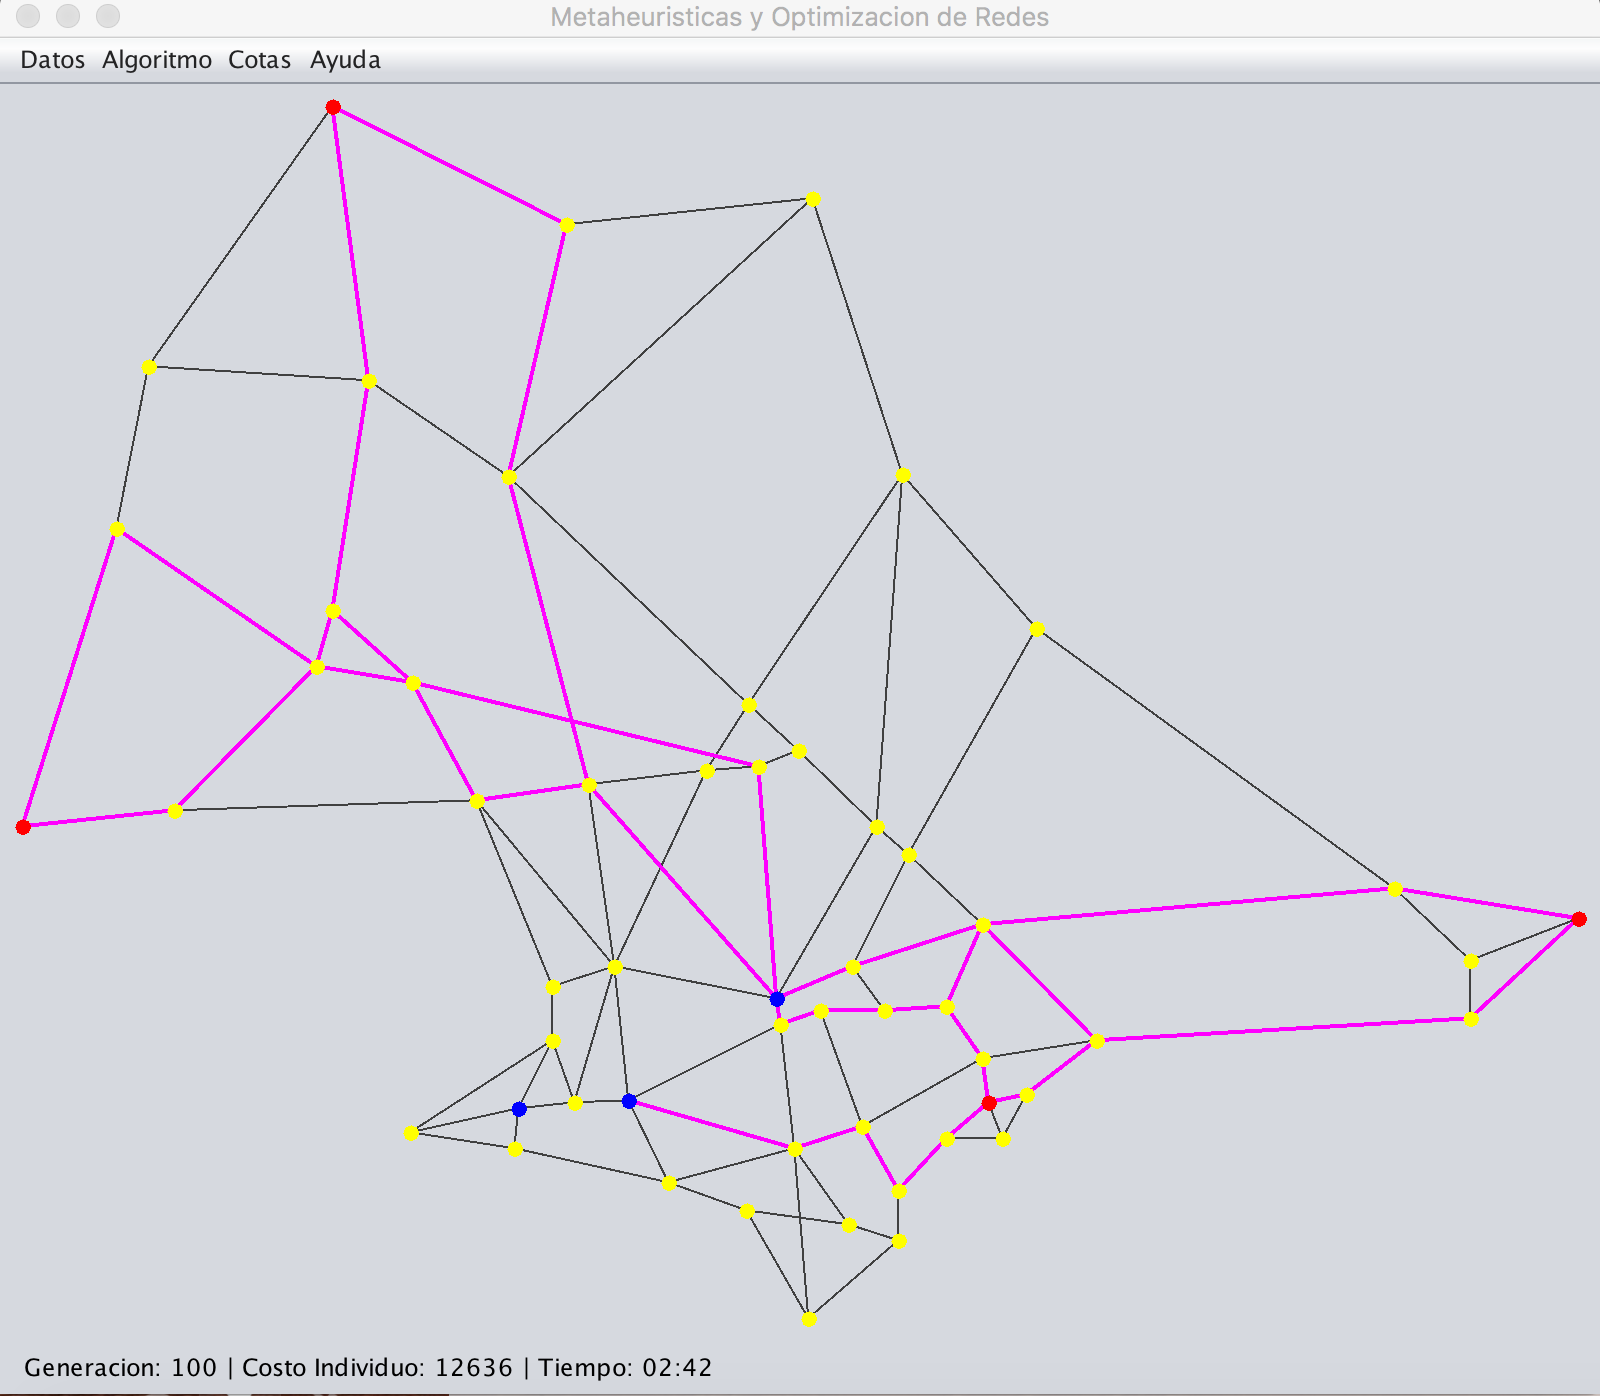
\includegraphics[scale=0.4]{img/metaheuristica/i1_s1}
\end{center}

\textbf{Algoritmo2}:
\begin{center}
	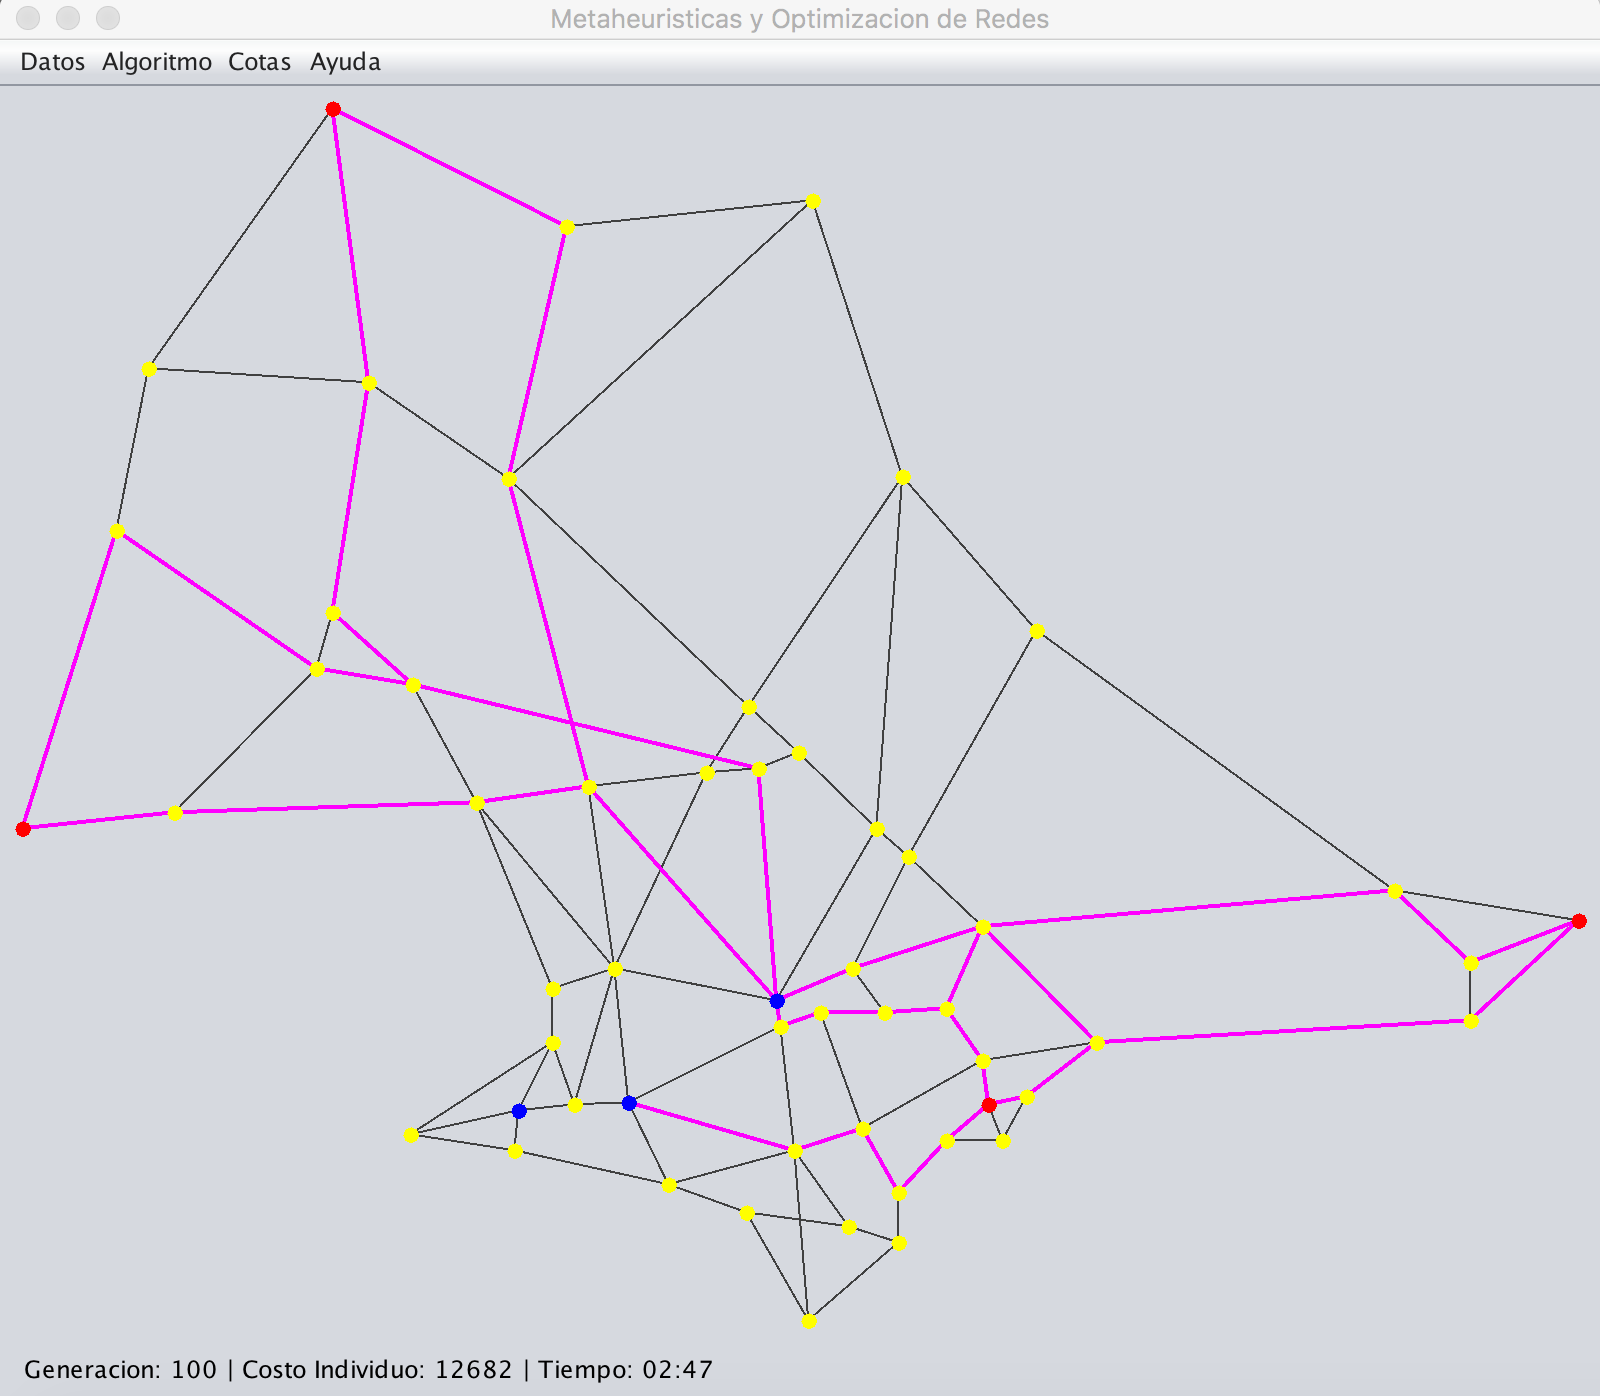
\includegraphics[scale=0.4]{img/metaheuristica/i1_s2}
\end{center}

\textbf{Algoritmo3}:
\begin{center}
	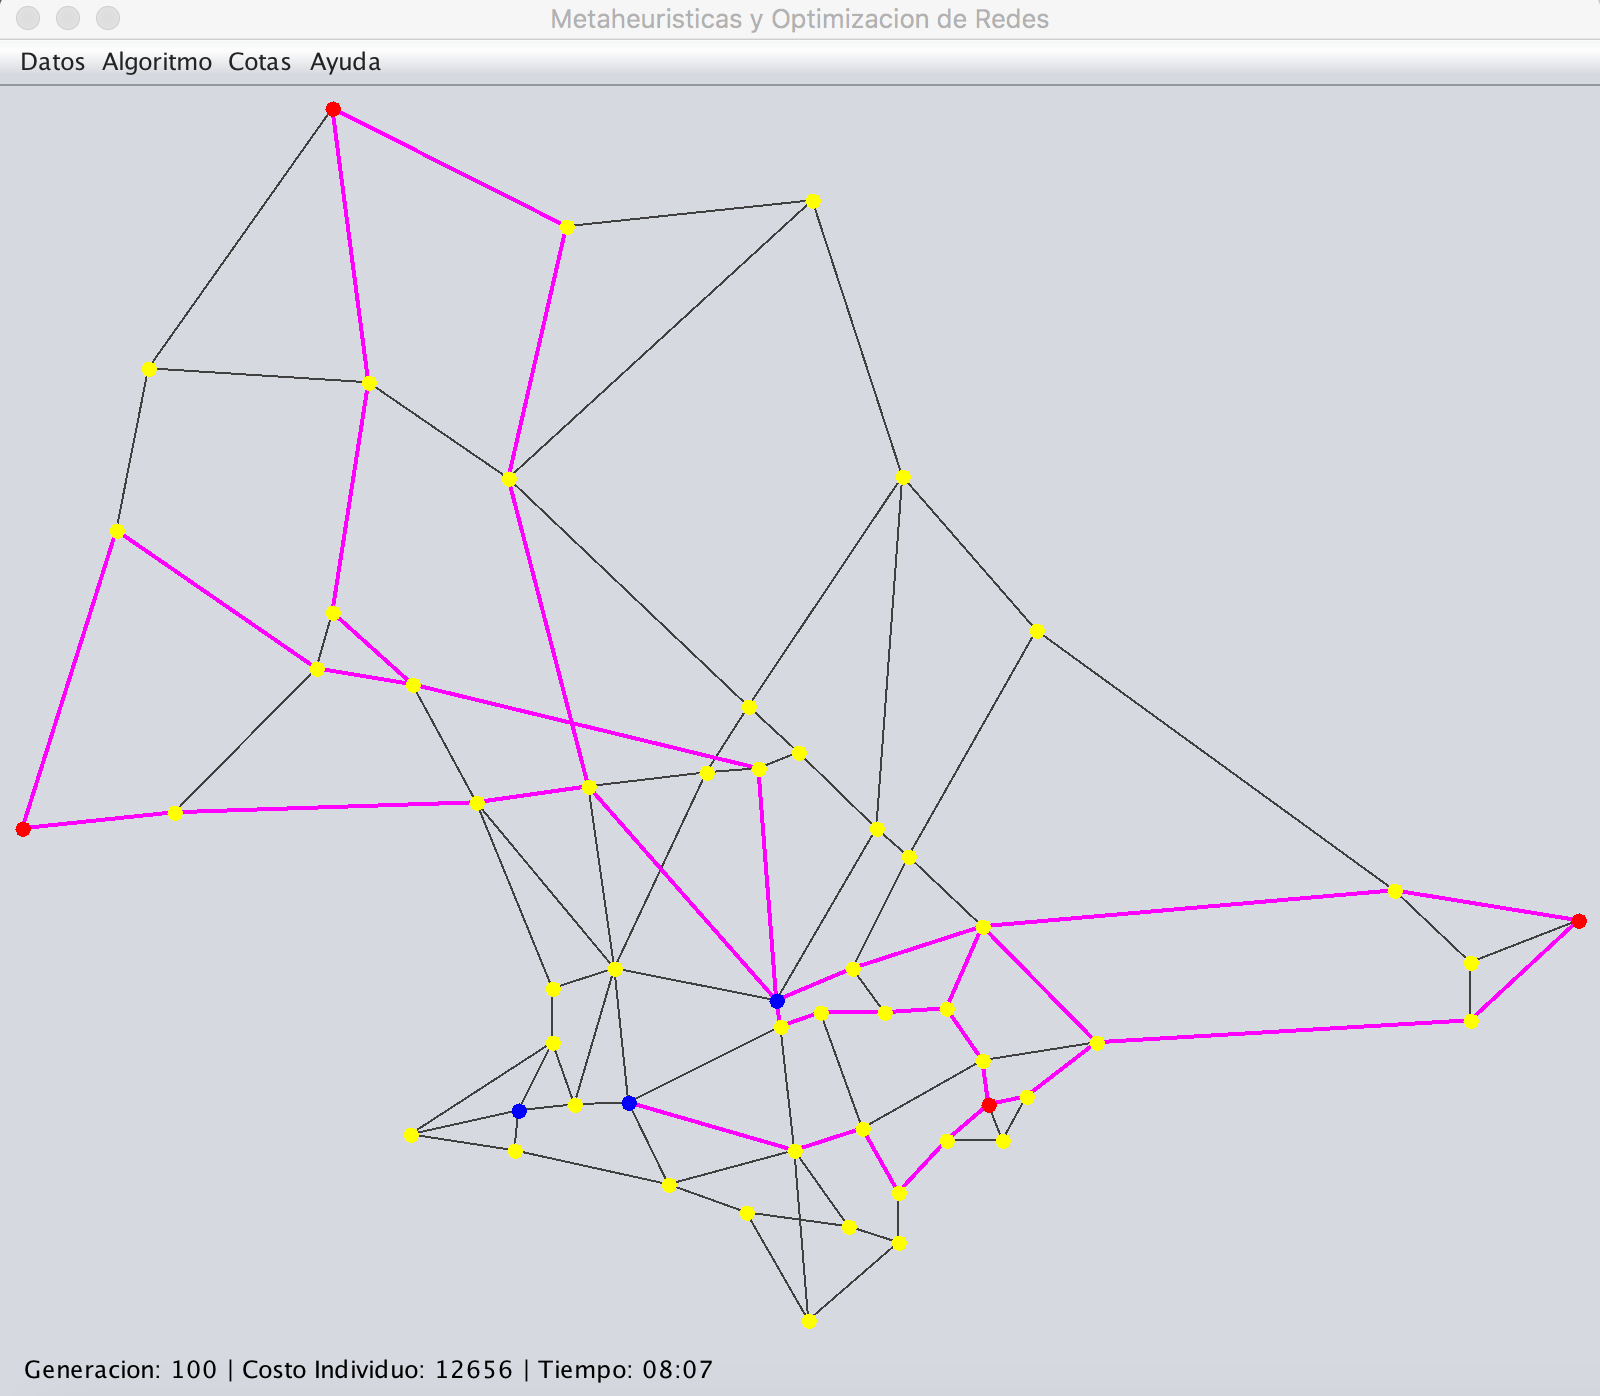
\includegraphics[scale=0.4]{img/metaheuristica/i1_s3}
\end{center}

\textbf{Algoritmo4}:
\begin{center}
	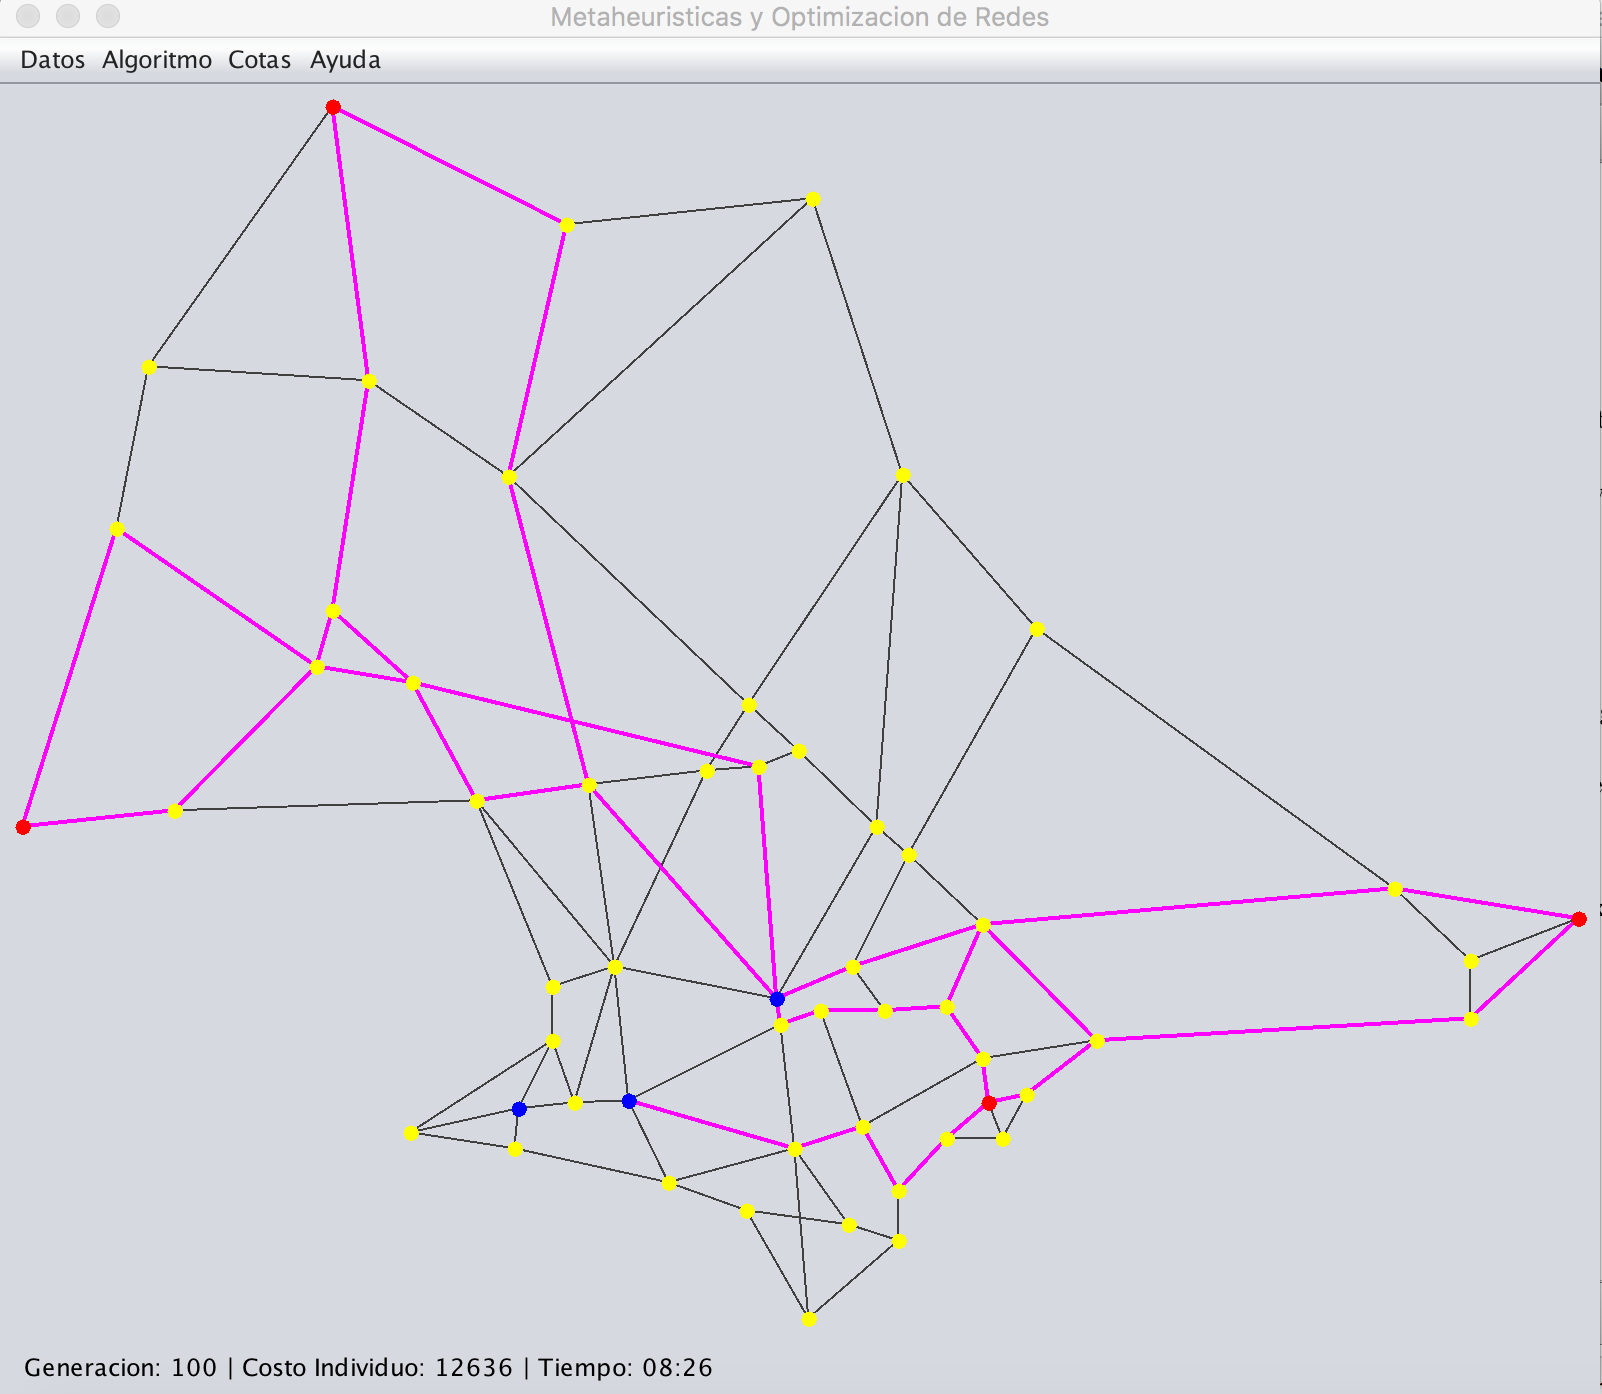
\includegraphics[scale=0.4]{img/metaheuristica/i1_s4}
\end{center}
\subsubsection{Instancia II}
Los resultados que se reportan a continuación comparten la siguiente configuración:
\begin{itemize}
	\item Ruido permitido en inicialización y mutación: 0-100.
	\item Tamaño de la población: 500
	\item Cantidad de generaciones: 150
	\item Probabilidad de cruzamientos por generación: 50\%
	\item Probabilidad de mutaciones por generación: 10\%
\end{itemize}

\textbf{Algoritmo1}:
\begin{center}
	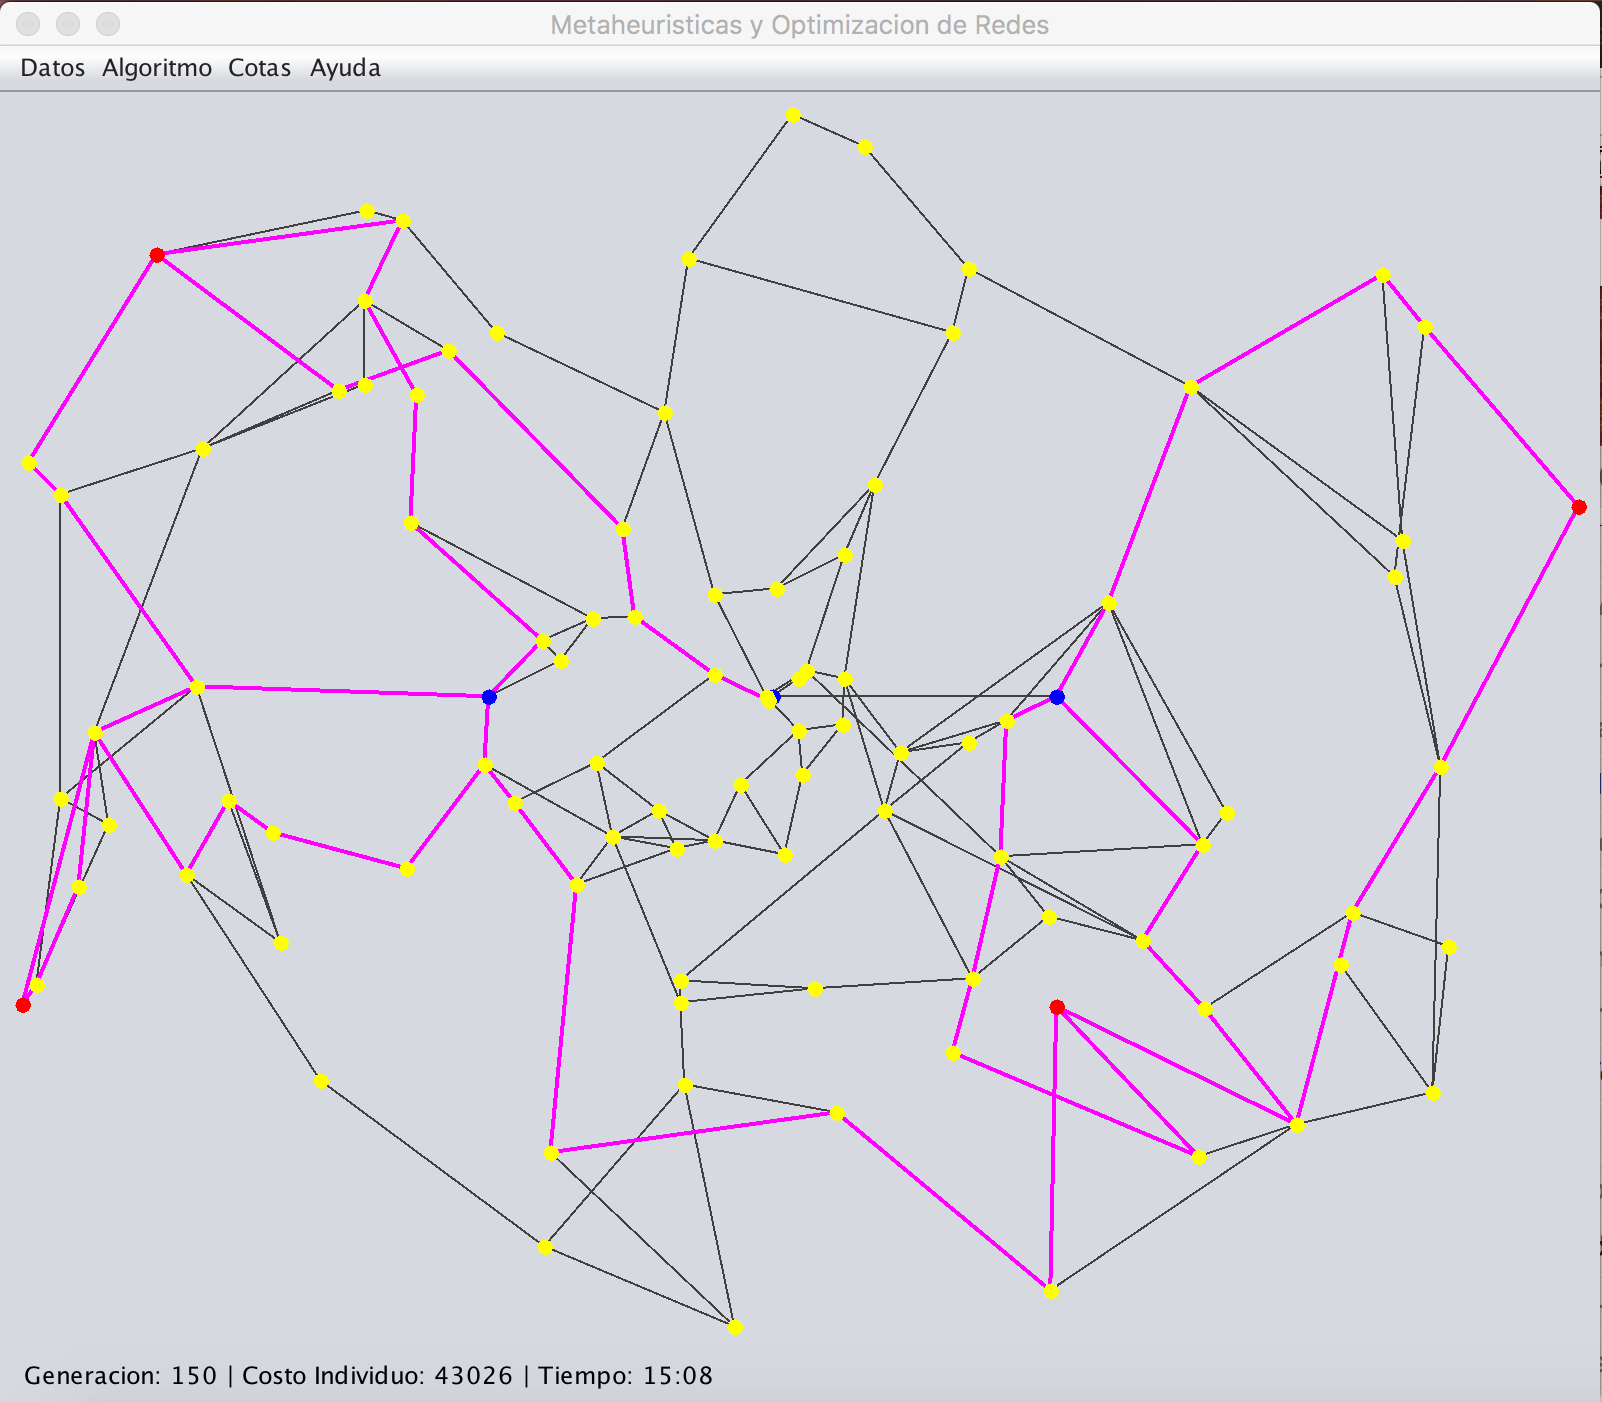
\includegraphics[scale=0.4]{img/metaheuristica/i2_s1}
\end{center}
\newpage
\textbf{Algoritmo4}:
\begin{center}
	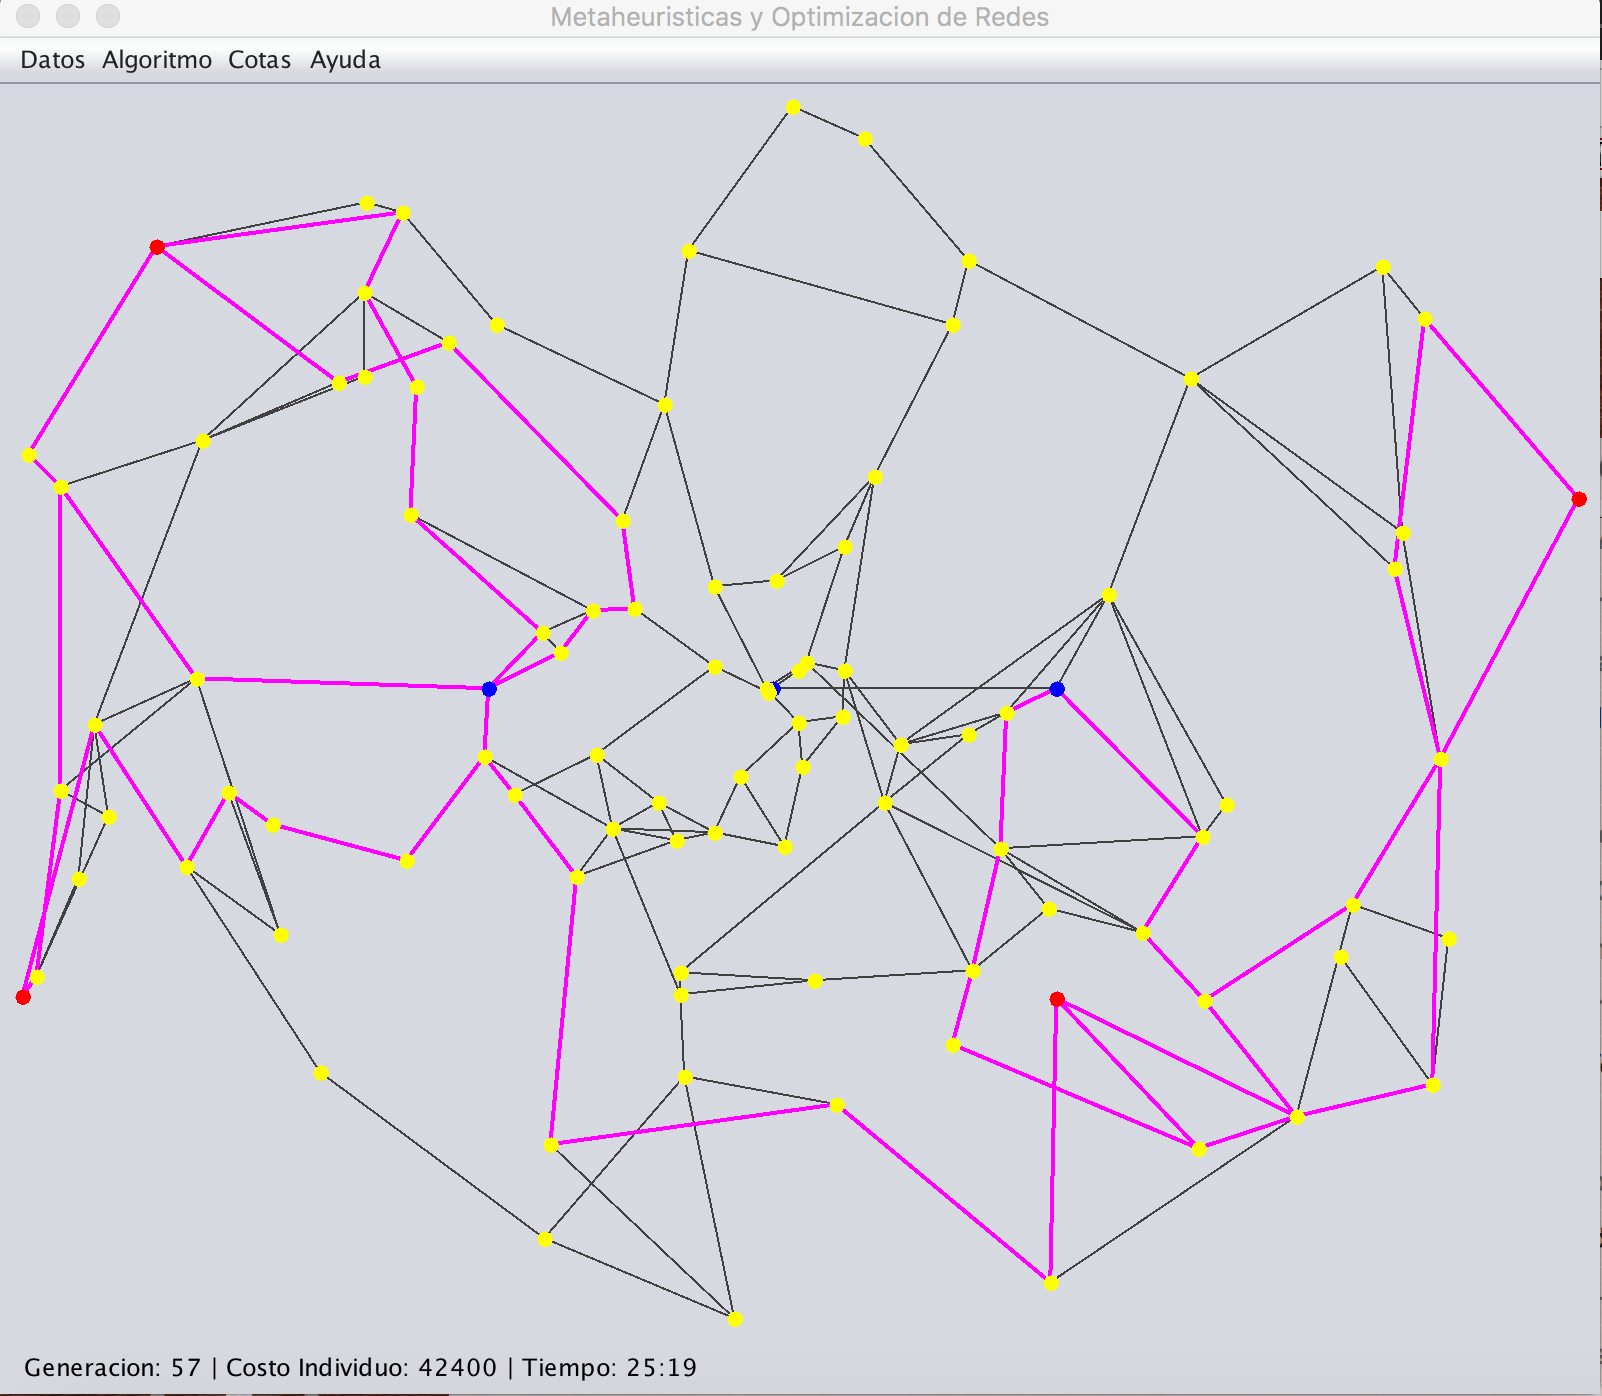
\includegraphics[scale=0.4]{img/metaheuristica/i2_s4}
\end{center}

\subsubsection{Instancia III}
Los resultados que se reportan a continuación comparten la siguiente configuración:
\begin{itemize}
	\item Ruido permitido en inicialización y mutación: 0-100.
	\item Tamaño de la población: 200
	\item Cantidad de generaciones: 25
	\item Probabilidad de cruzamientos por generación: 50\%
	\item Probabilidad de mutaciones por generación: 10\%
\end{itemize}

Para esta intancia no se encontraron mayores dificultades en la búsqueda del mejor valor encontrado.
\newpage
\textbf{Algoritmo1}:
\begin{center}
	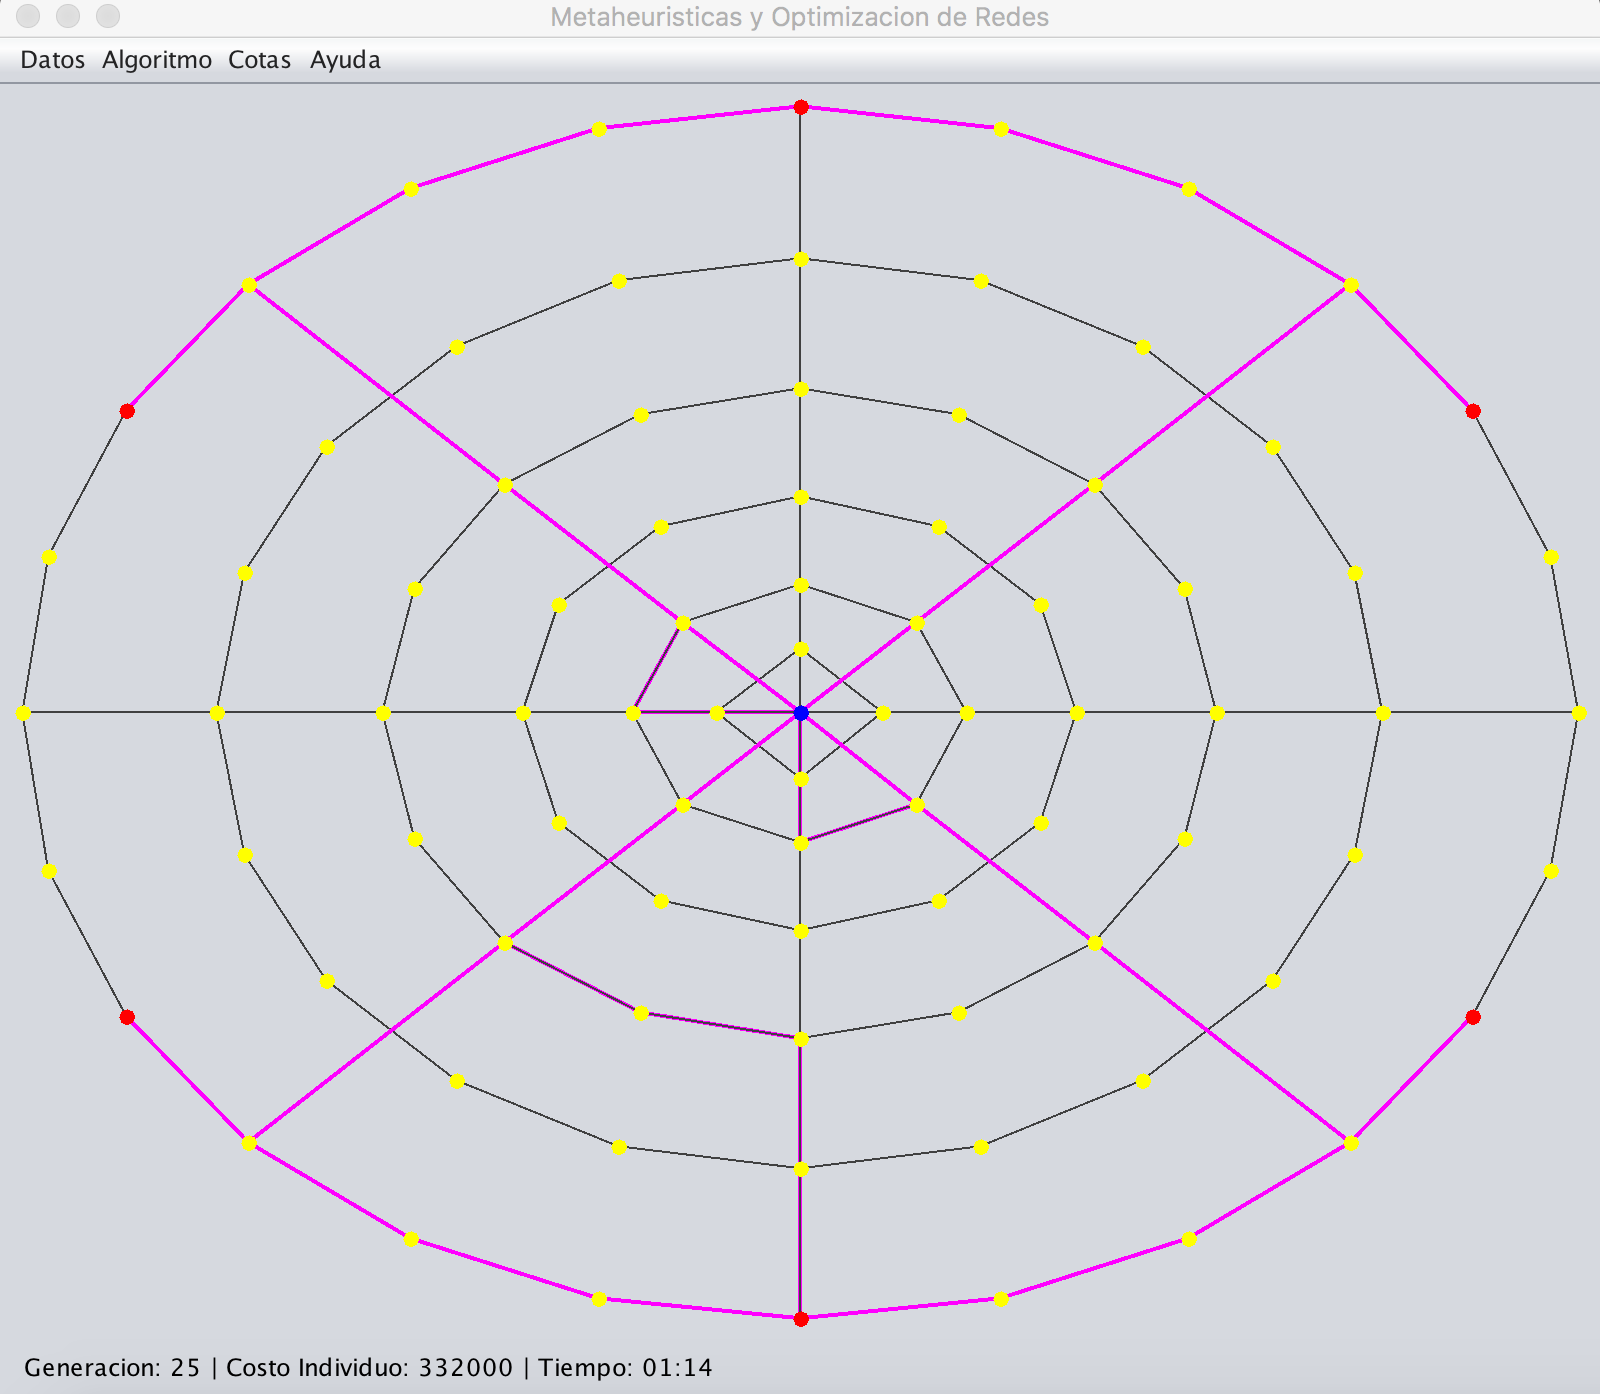
\includegraphics[scale=0.4]{img/metaheuristica/i3_s1}
\end{center}

\textbf{Algoritmo2}:
\begin{center}
	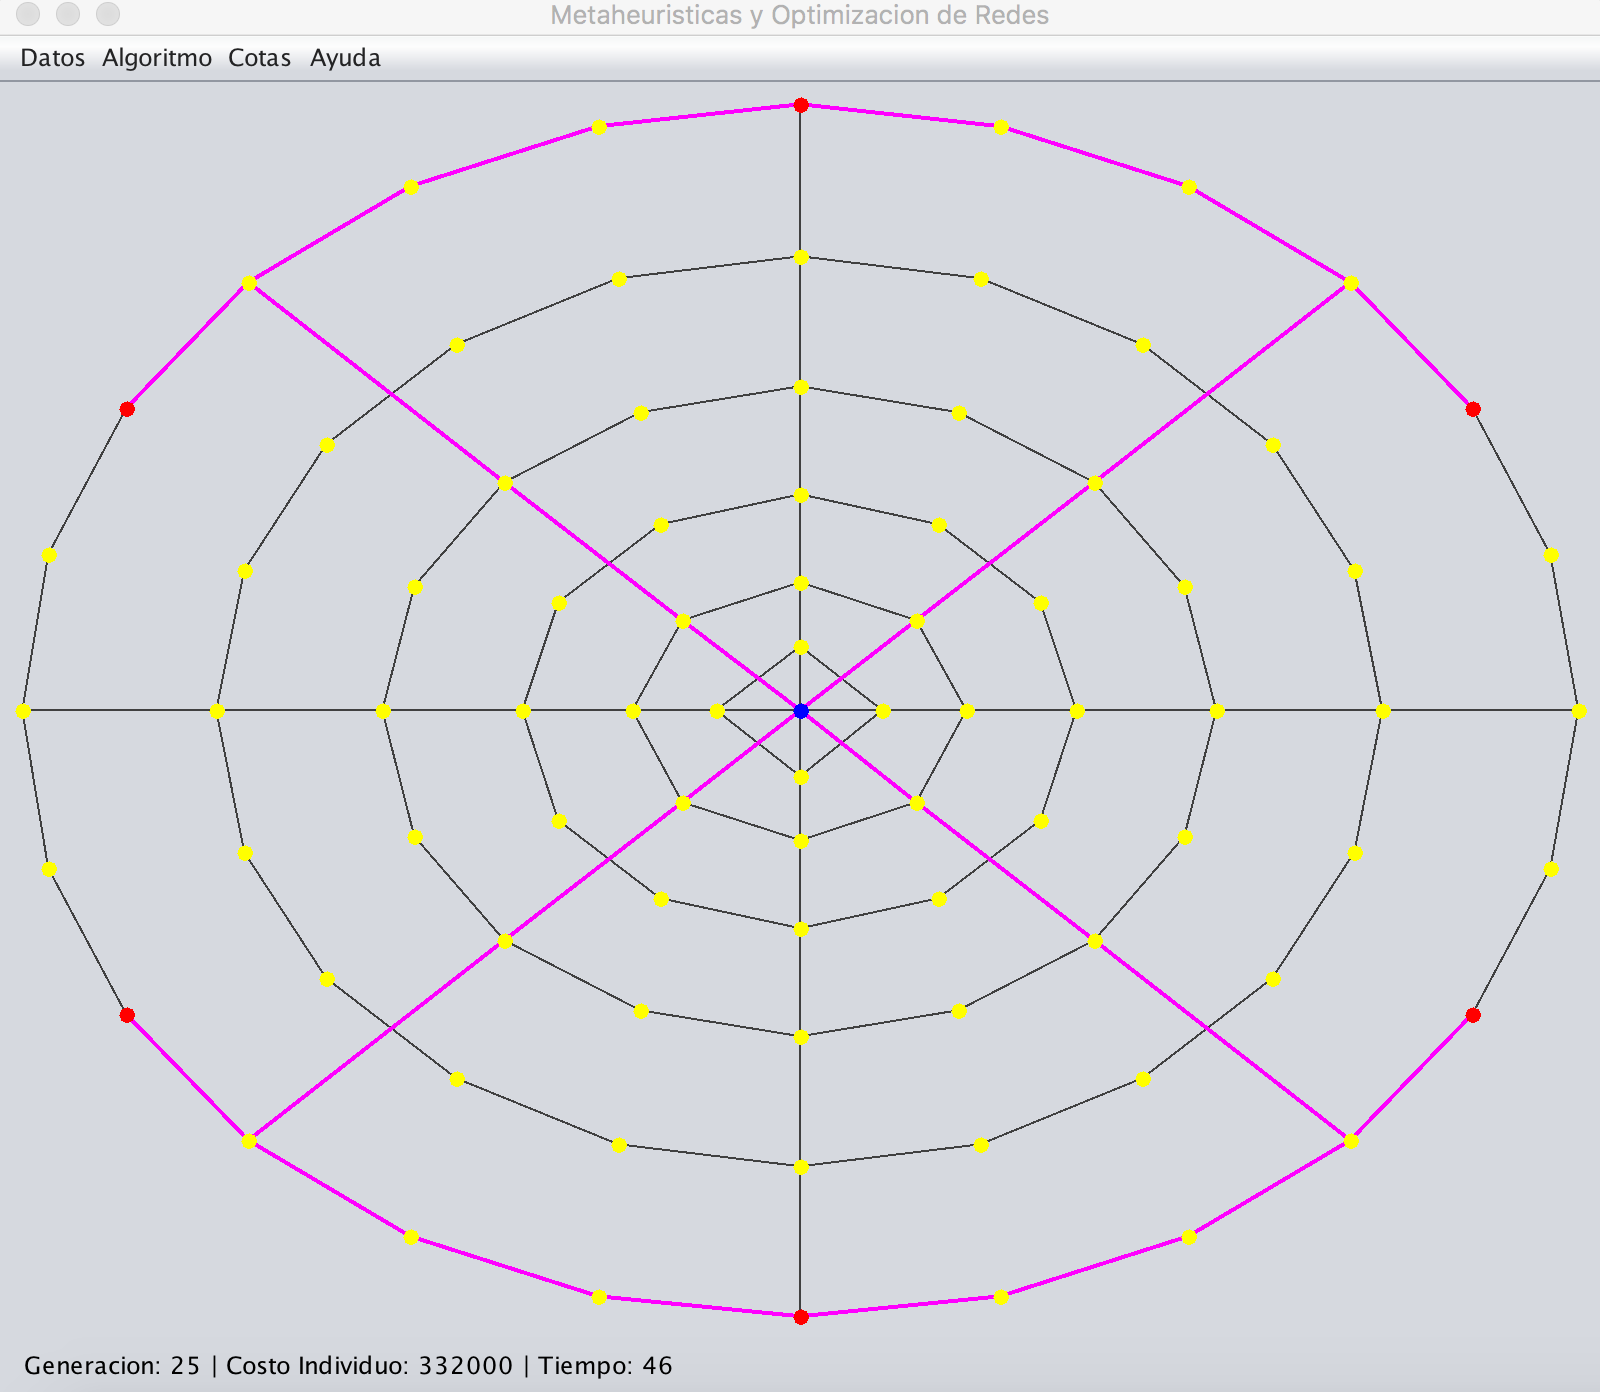
\includegraphics[scale=0.4]{img/metaheuristica/i3_s2}
\end{center}

\textbf{Algoritmo3}:
\begin{center}
	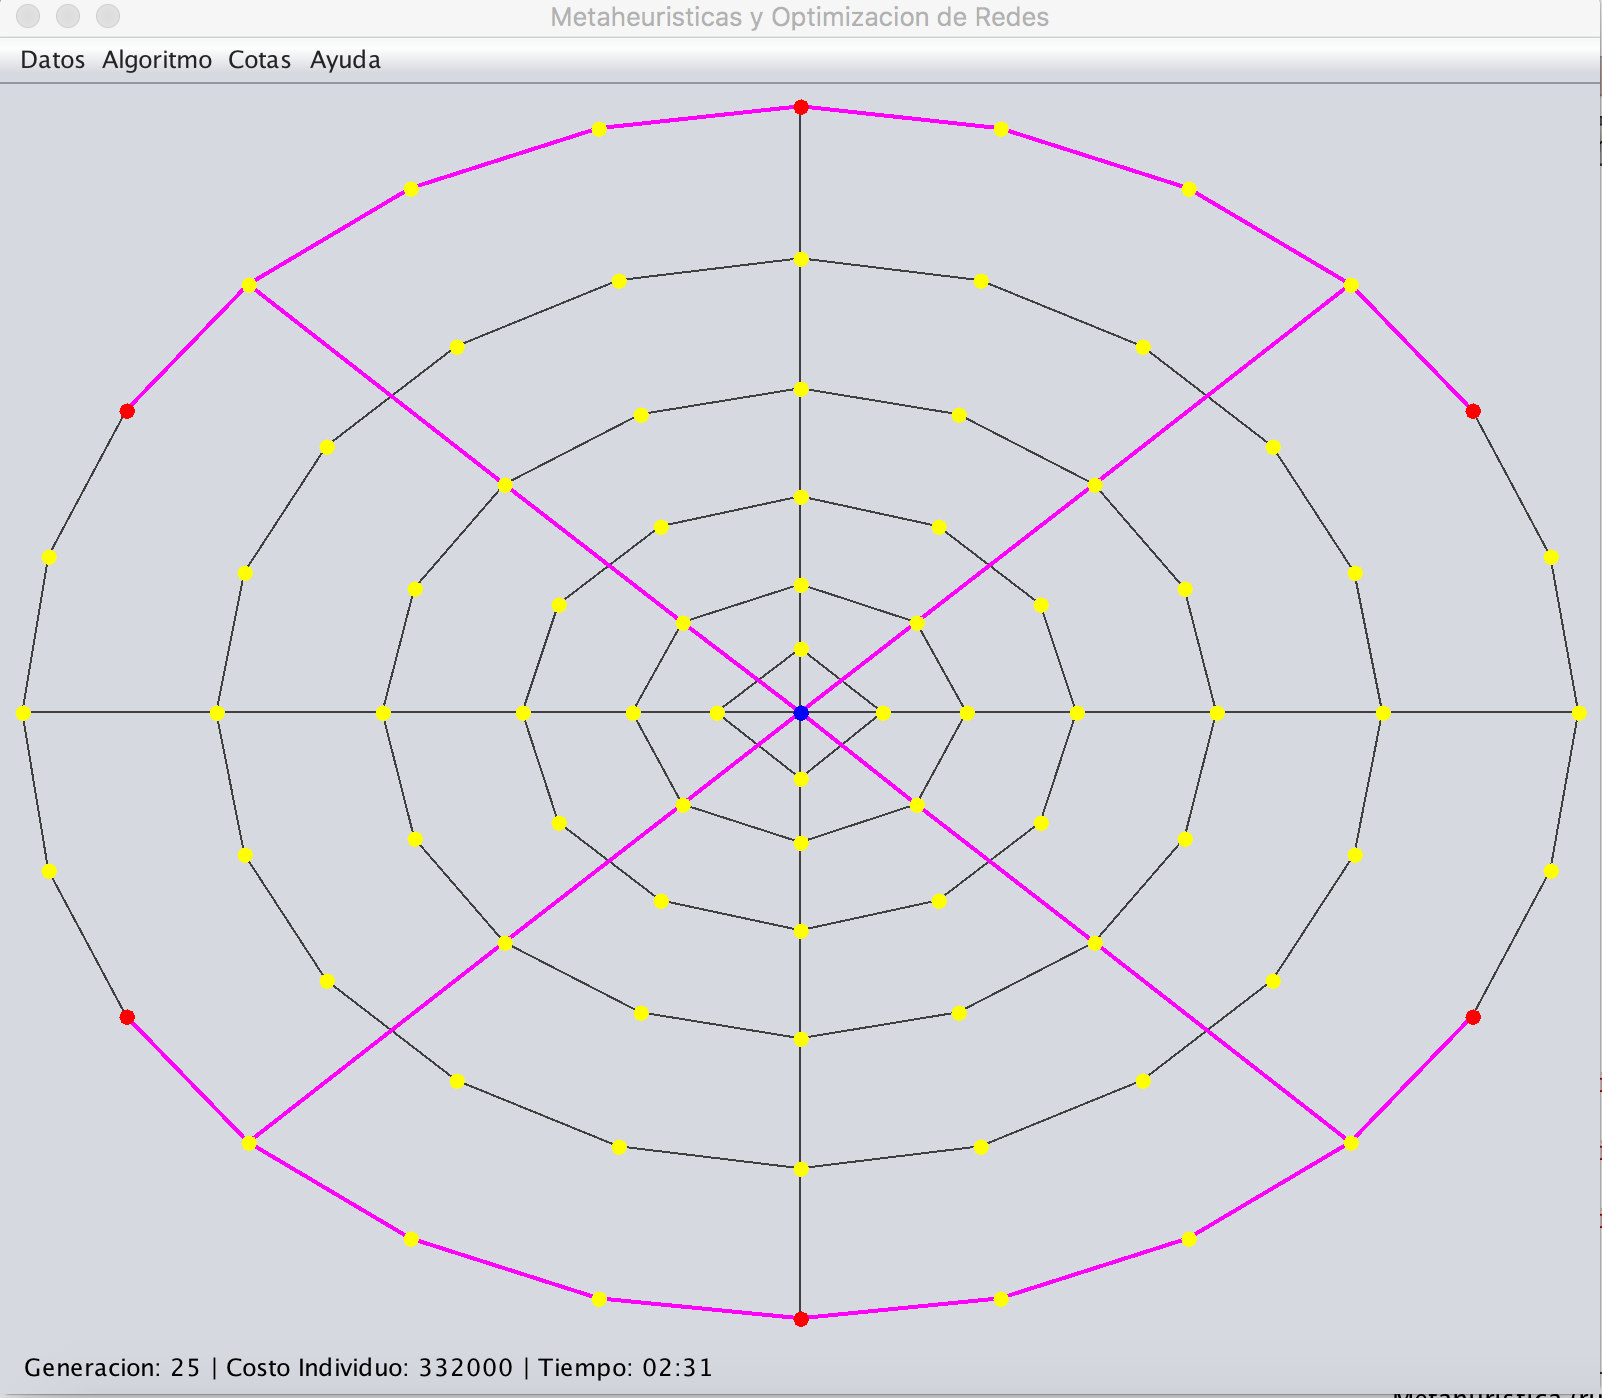
\includegraphics[scale=0.4]{img/metaheuristica/i3_s3}
\end{center}

\textbf{Algoritmo4}:
\begin{center}
	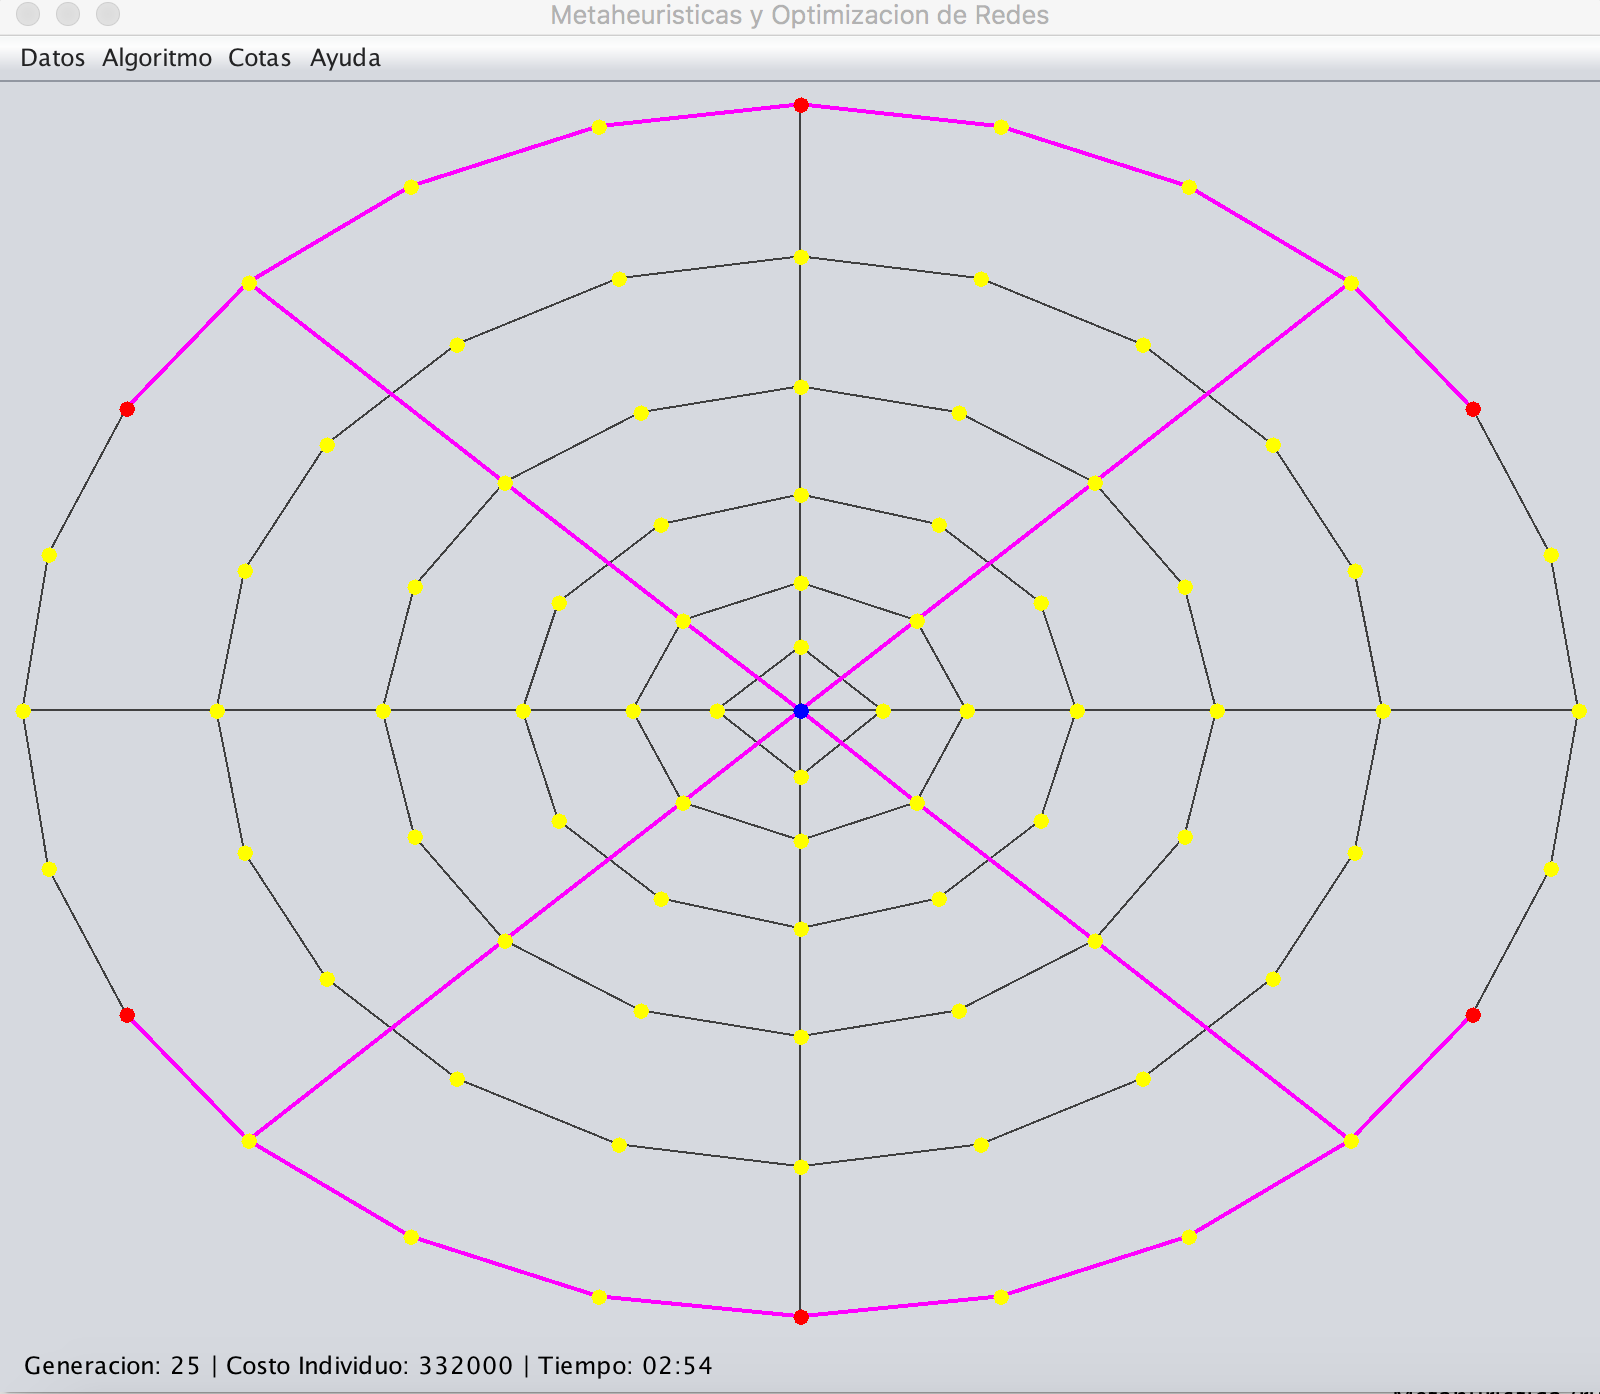
\includegraphics[scale=0.4]{img/metaheuristica/i3_s4}
\end{center}

\subsection{Conclusiones}
Considerando que los márgenes de errores estuvieron cercanos al 25\% en los mejores casos y que las ejecuciones de la metaheurística resultaron sensiblemente menores que las de su contraparte exacta la evaluación general resulta ampliamente satisfactoria.

En el proceso de implementación se fueron incorporando algoritmos de selección para poder atacar el problema de convergencias tempranas a óptimos locales. Dichos algoritmos permitieron validar dicha hipótesis y mejorar sustantivamente los resultados encontrados. En particular esto se evidenció más fuertemente en la instancia II en donde con el algoritmo4 fue posible encontrar de manera reiterada valores por debajo del mejor costo que que los que se encontraban con el algoritmo1.

Por otra parte en lo que respecta los operadores de cruzamiento y mutación, ambos resultaron efectivos y eficientes como se mencionó anteriormente. Esta situación permitió centrar los ajustes de la metaheurística en el proceso de selección y acortar la cantidad de ajustes para las diferentes instancias reduciéndolos prácticamente que a la cantidad de la población y al criterio de parada para generaciones invariantes.

En definitiva, en este Obligatorio no sólo se logró entender el trabajo con metaheurísticas desde una perspectiva teórica y práctica sino que también se atacaron distintos problemas inherentes a la utilización de una en particular.

\section{Referencias consultadas}
\begin{thebibliography}{99}		
	\bibitem{1} Alves Pessoa, et. al. Robust constrained shortest path problems under budgeted uncertainty.
	
	\bibitem{2} Ziegelmann, M. Constrained Shortest Path and Related Problems. Universitat der Saarlandes. \\
	\url{http://scidok.sulb.uni-saarland.de/volltexte/2004/251/pdf/MarkZiegelmann_ProfDrKurtMehlhorn.pdf}
	
	\bibitem{3} Lecture Notes: Solving linear and integer programs using the GNU linear programming kit.  Duke University. \\ \url{https://www.cs.duke.edu/courses/spring08/cps296.2/solvers.pdf}
	
	\bibitem{4} Lecture Notes: Integer Programming, Relaxations and Bounds. Technische Universitat Kaiserslautern. \\
	\url{http://www.mathematik.uni-kl.de/fileadmin/AGs/opt/Lehre/WS1314/IntegerProgramming_WS1314/ip-chapter6.pdf}
	
	\bibitem{5} Lecture Notes: The KnapSack Problem. University of Texas at Dallas. \\
	\url{https://www.utdallas.edu/~scniu/OPRE-6201/documents/DP3-Knapsack.pdf}
	
\end{thebibliography}

\newpage
\section{Anexo I: Pruebas realizadas}
\subsection{Cálculo de cotas y factibilidad de la población inicial}

A efectos de establecer las cotas de los delays para la parte IV, se resolvió el problema de maximizar el delay para un camino a partir de las soluciones de la parte I. Obteniendo como cotas superiores los valores 1263, 1187, 841 y 1263 para Carrasco, Cerro, Pocitos y Colón respectivamente.
 
A continuación se muestran a la izquierda las líneas del individuo I y a la derecha las del individuo II.
\begin{flushleft}
	Líneas de CAR:
\end{flushleft}
\begin{align*}
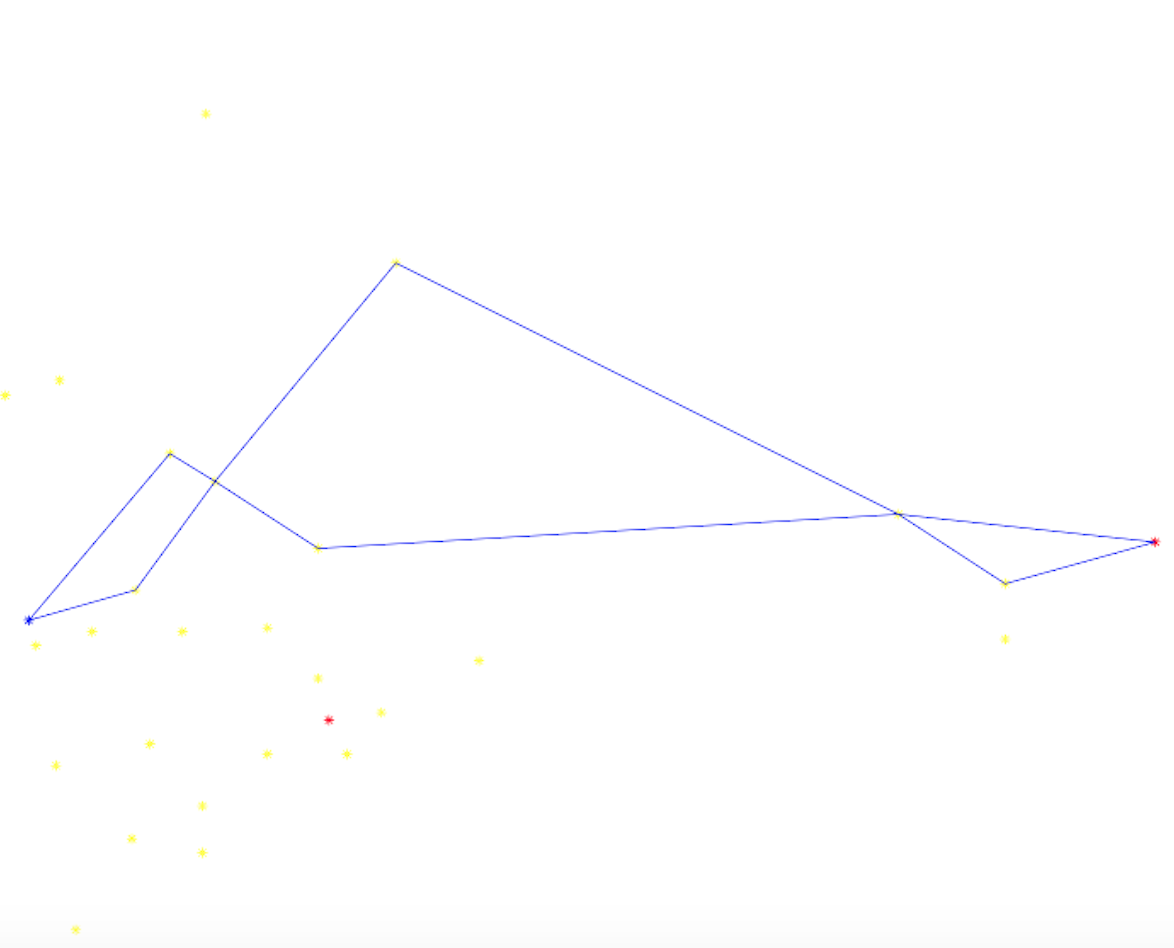
\includegraphics[scale=0.25]{img/ind/parciales/4-2.png}
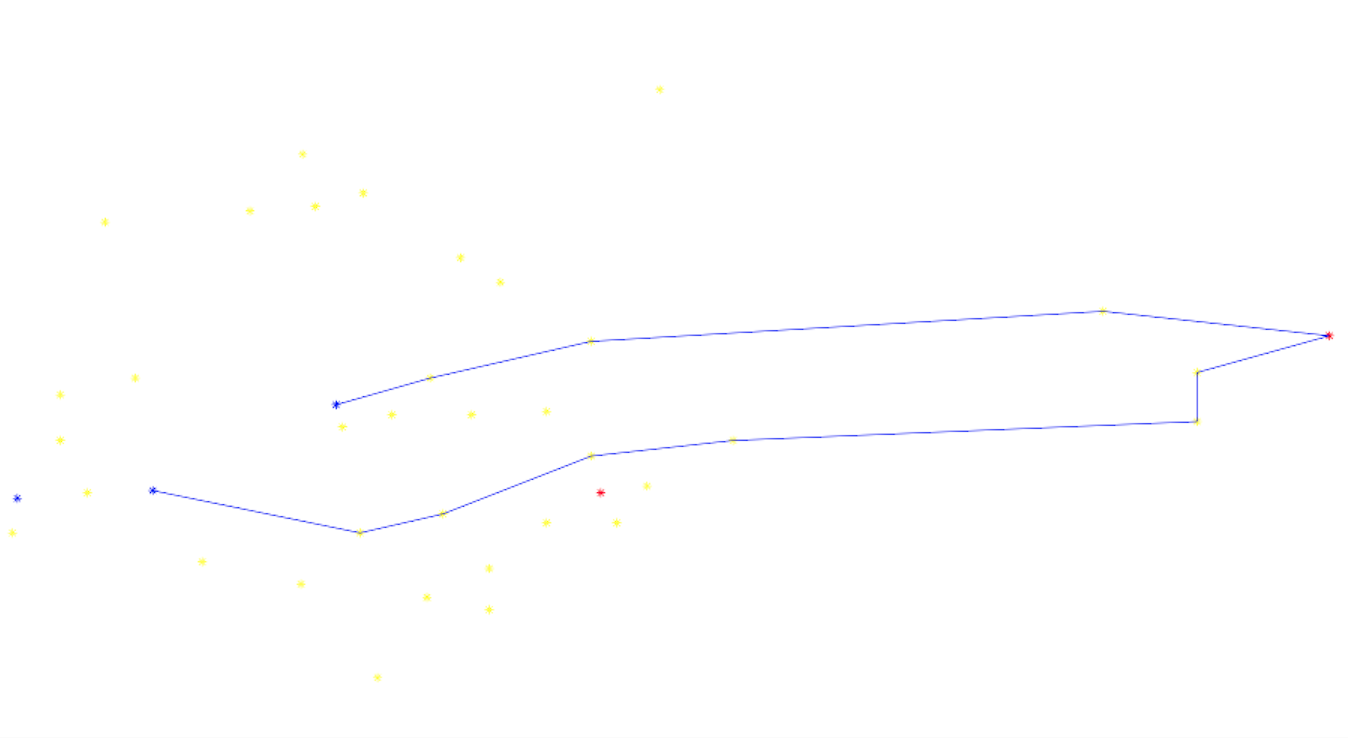
\includegraphics[scale=0.25]{img/ind/parciales/4-4.png}
\end{align*}
\begin{flushleft}
	Líneas de CRO:
\end{flushleft}
\begin{align*}
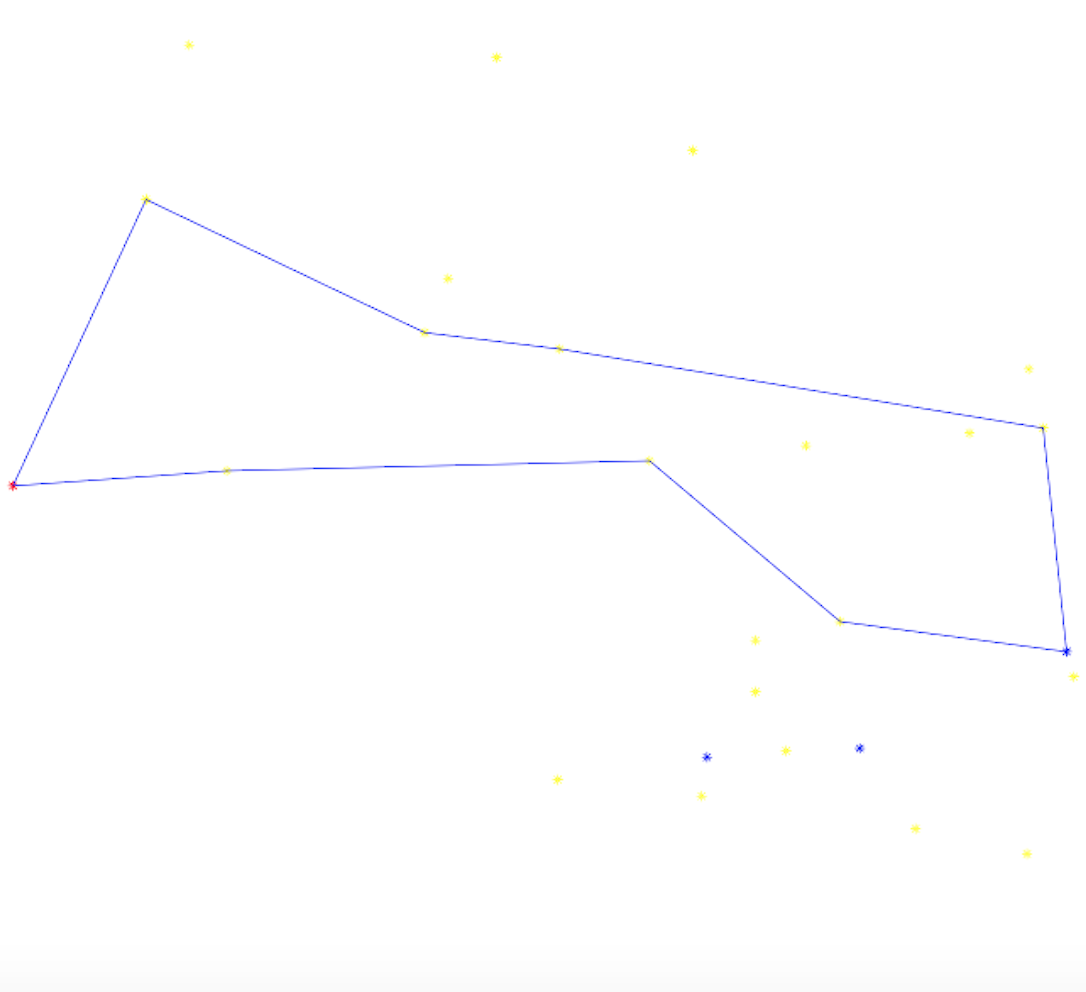
\includegraphics[scale=0.25]{img/ind/parciales/5-3.png}
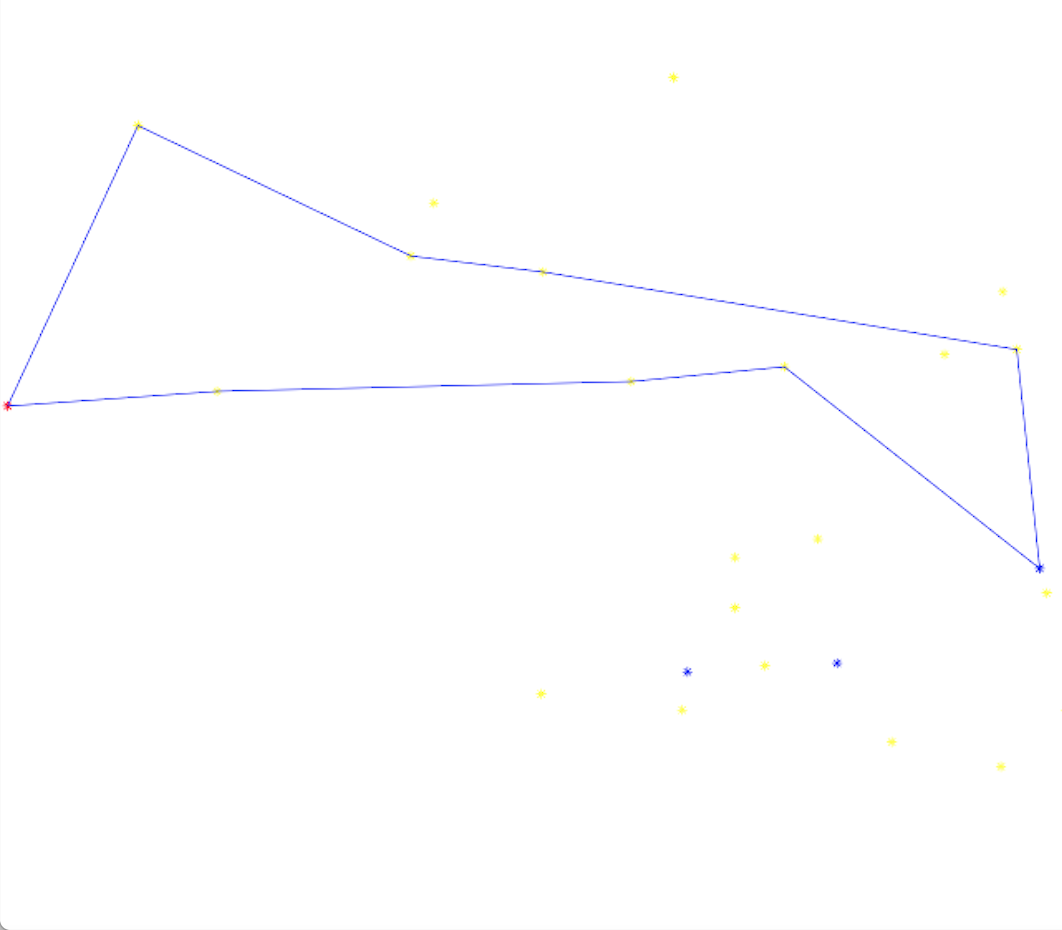
\includegraphics[scale=0.25]{img/ind/parciales/5-1.png}
\end{align*}
\begin{flushleft}
	Líneas de POC:
\end{flushleft}
\begin{align*}
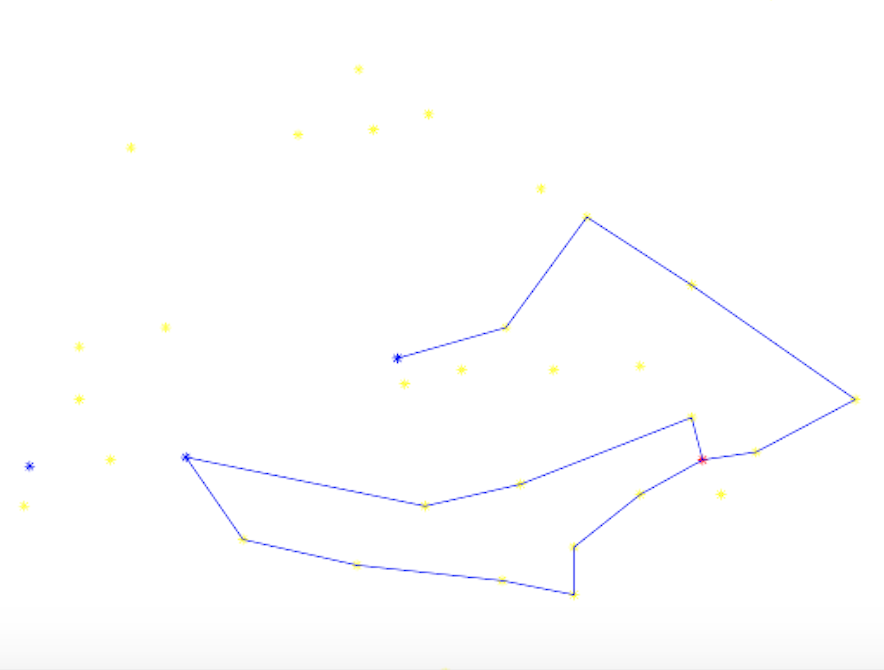
\includegraphics[scale=0.3]{img/ind/parciales/6-2.png}
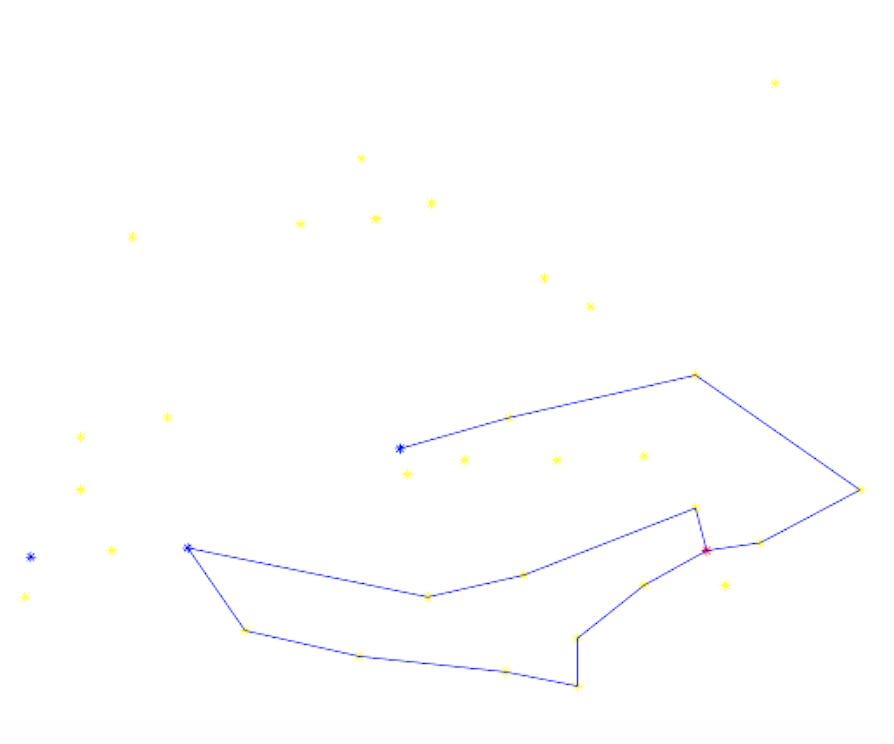
\includegraphics[scale=0.3]{img/ind/parciales/6-1.png}
\end{align*}
\begin{flushleft}
	Líneas de TCO:
\end{flushleft}
\begin{align*}
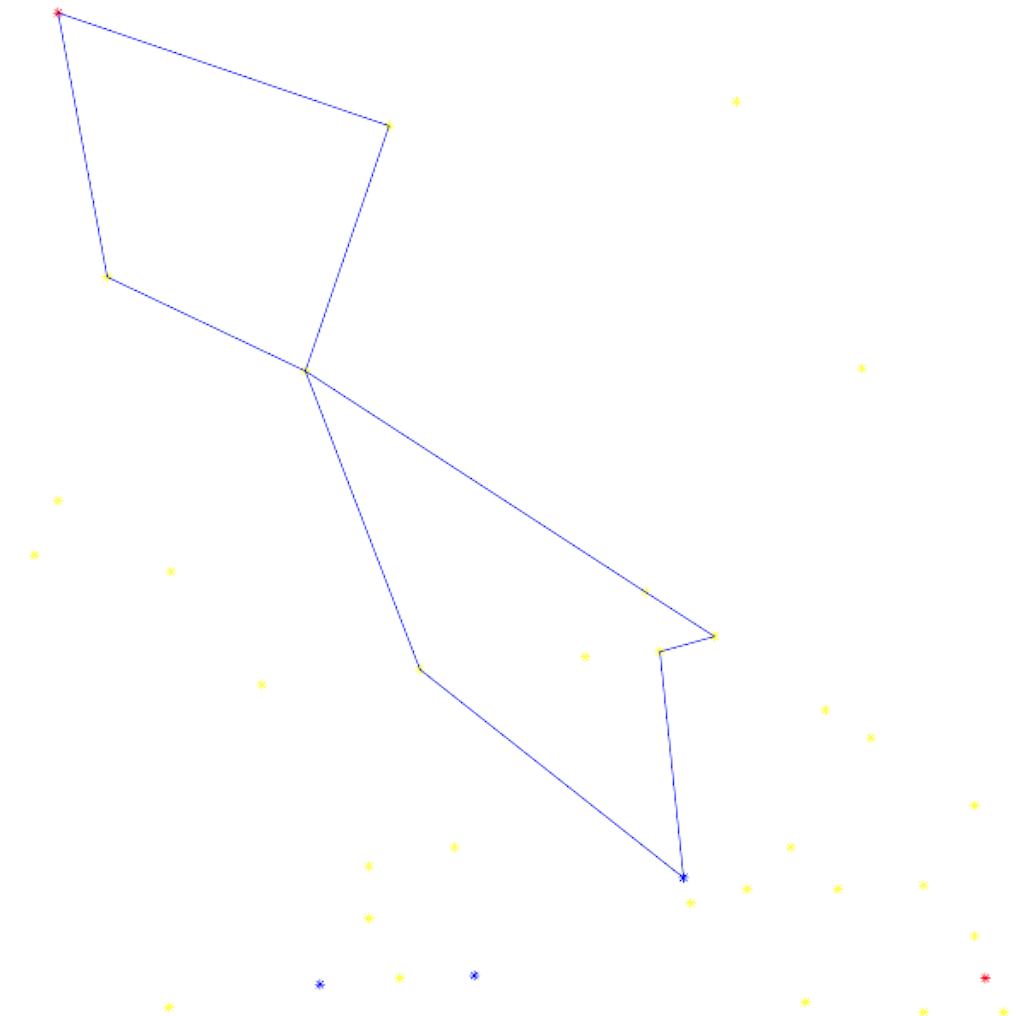
\includegraphics[scale=0.25]{img/ind/parciales/7-1.png}
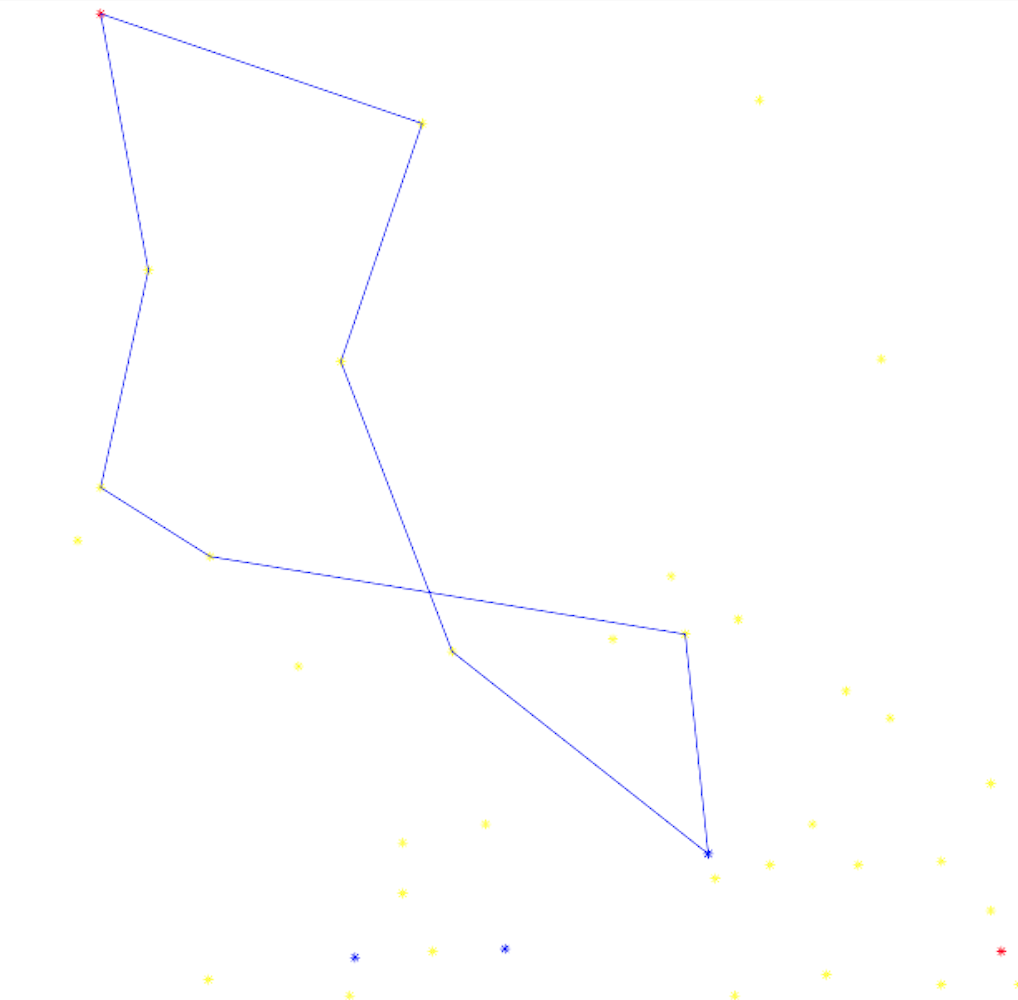
\includegraphics[scale=0.25]{img/ind/parciales/7-2.png}
\end{align*}
 Individuo I y II respectivamente:
 \begin{align*}
 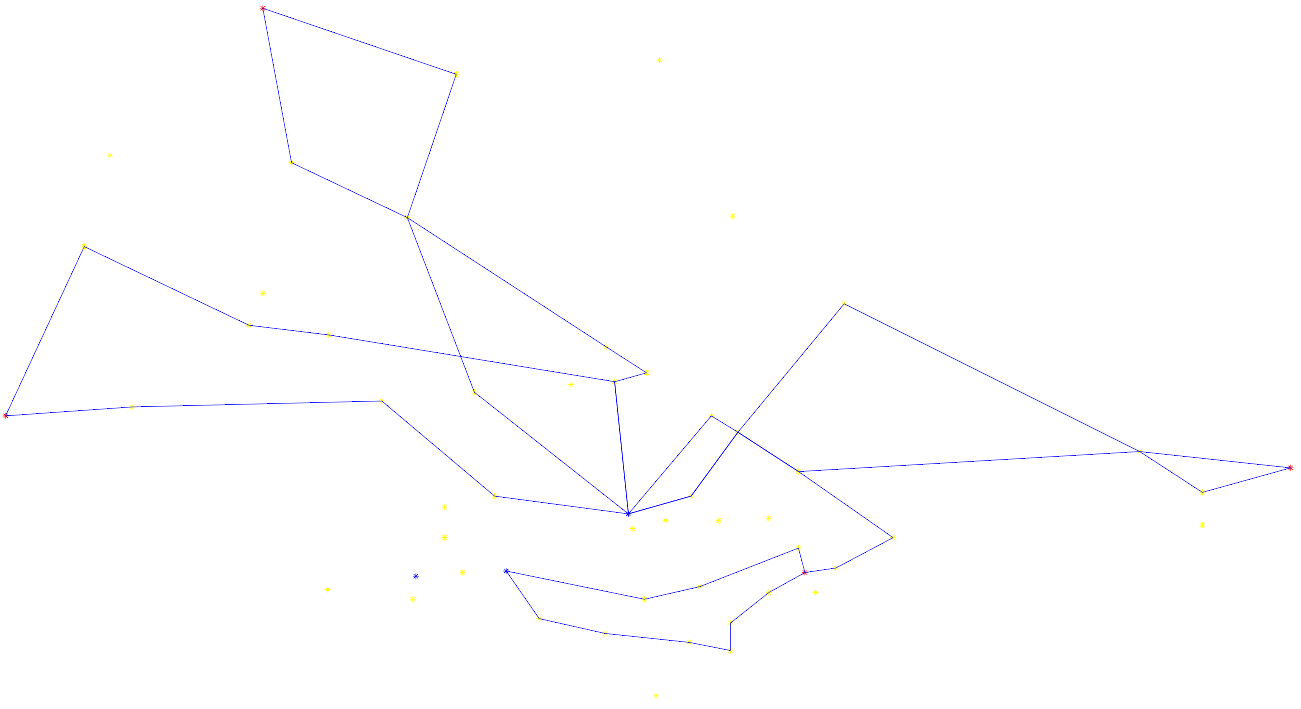
\includegraphics[scale=0.3]{img/ind/2321N.png}
 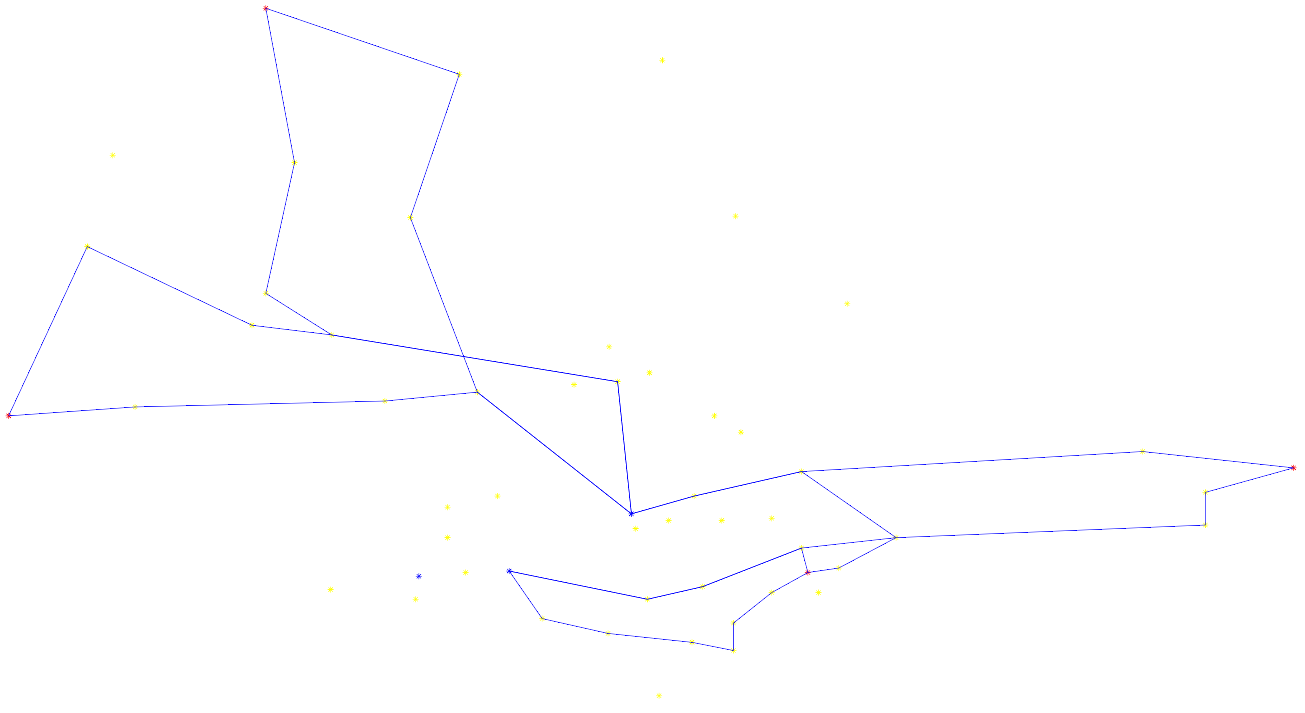
\includegraphics[scale=0.3]{img/ind/4112N.png}
 \end{align*}
 \begin{flushleft}
 Finalmente se adjuntan otros dos individuos obtenidos a partir del mismo proceso:
 \end{flushleft}
\begin{align*}
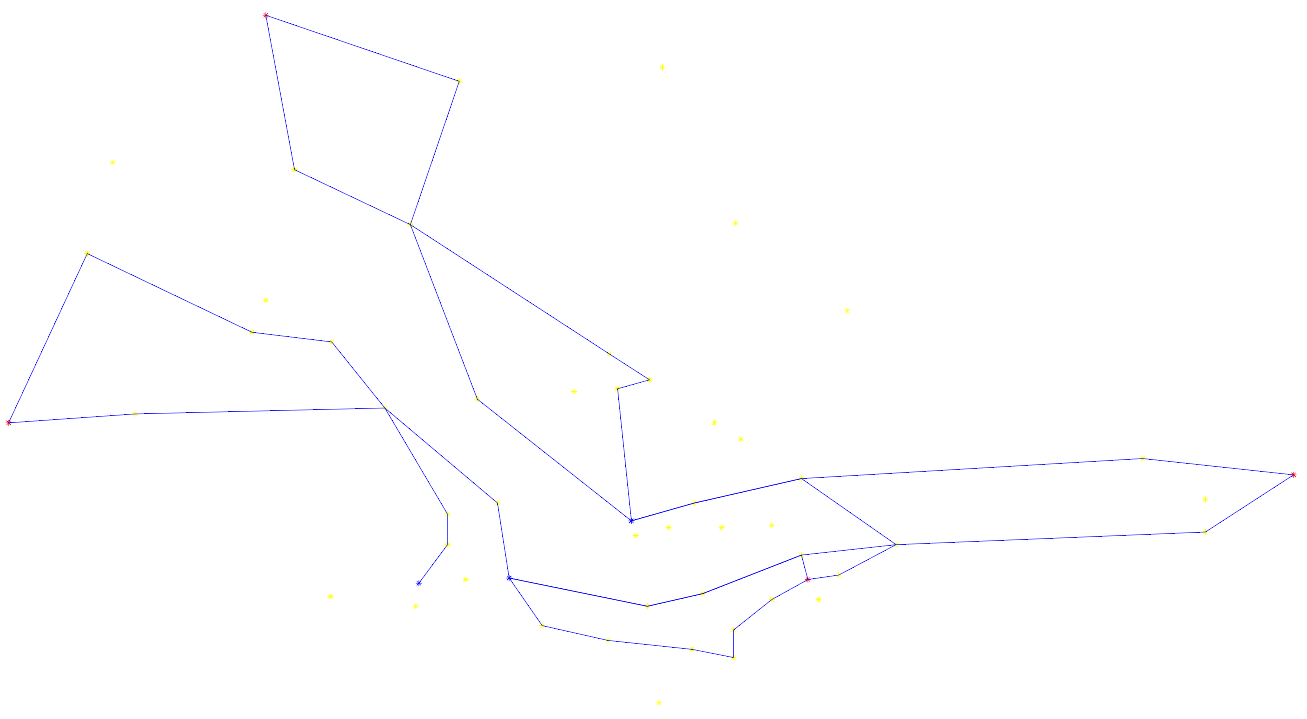
\includegraphics[scale=0.3]{img/ind/3211.png}
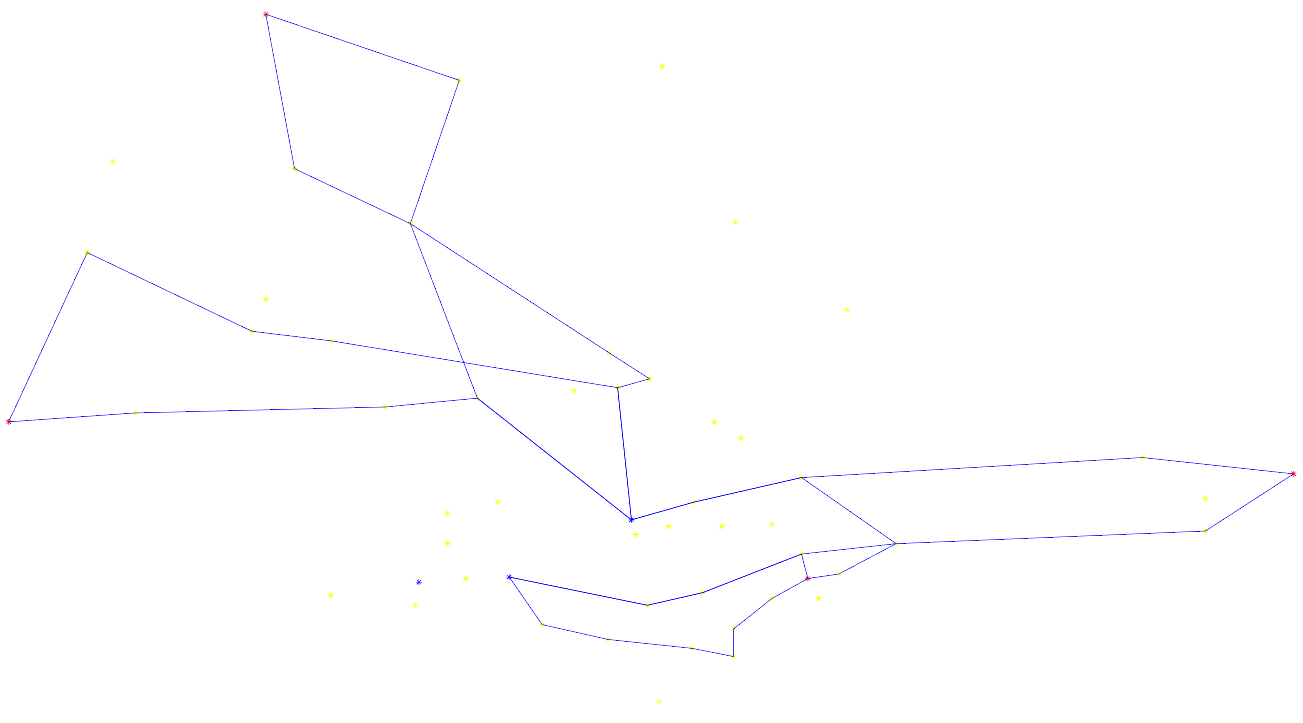
\includegraphics[scale=0.3]{img/ind/3111.png}
\end{align*}

\newpage
\section{Anexo II: Acerca de las implementaciones realizadas}
\subsection{Introducción}
Para las partes I, II y III se programaron scripts en Octave que se encuentran en los directorios Parte1, Parte2 y Parte3 del entregable que acompaña este informe.
Además se cuenta con directorios auxiliares o comunes que son, ``datos'' y ``out'', encargados de almacenar la entrada o salida de los scripts.

Cabe alcarar que al utilizar un lenguaje de scripting algunas funcionalidades se encuentran harcodeadas siendo que por simplicidad pueden configurarse directamente desde desde cada script.

En general todas las partes cuentan con unos scripts llamados \textbf{carga}, \textbf{adaptador}, \textbf{toGLPK} y \textbf{parteX} cuyas funcionalidades son:
\begin{itemize}
	\item \textbf{carga}:  Lee los archivos de aristas y nodos correspondientes. Los nombres de los archivos son pasados por parámetro retornando estructuras bien separadas; nodos, aristas, coordenadas, costos y delays.
	\item \textbf{adaptador}: Recibe como parámetro los nodos y aristas para luego retornar una matriz de adyacencia y un vector auxiliar para mejorar el acceso a la matriz.
	\item \textbf{toGLPK}: Octave cuenta con GLPK en sus librerias y el mismo recibe un formato de los parámetros particular. En esta función transformamos nuestra matriz de adyacencia y restricciones conocidas a un problema lineal que GLPK pueda ejecutar y lo ejecutamos retornando así el valor óptimo y las aristas que utilizó. Recibe como parámetro la matriz de adyacencia antes mencionada, el vector auxiliar, el vector de costos/delays y una lista de nodos especiales, pensando ya en generalizar el problema. Se hicieron pruebas de maximización por eso además opcionalmente puede recibir como parámetro el sentido de la optimizacion.
	\item \textbf{parteX}: Si bien para cada parte se hicieron scripts dedicados, en términos generales los scripts de este tipo utilizan un mismo esqueleto, cargan los datos, los adapta a la forma en la que se manipularán, se transforma a formato glpk, se ejecuta y se optienen los valores. Además contiene código para dibujar las soluciones y guardar la salida en el directorio ``out''. Los nombres de los archivos de aristas y nodos se encuentran harcodeados en este código.
\end{itemize}
\newpage
\subsection{Parte I}
El script implementado para esta parte puede recibir un parametro entero (1, 2 o 3) que le indicará que modo ejecutar y su fichero correspondiente es el archivo parte1.m

Ejecución:
\begin{itemize}
	\item parte1(1) - minimza costos.
	\item parte1(2) - minimza delays.
	\item parte1(3) - crea un CCM para cada fuente.
\end{itemize}


\subsection{Parte II}
En este caso, el script implementado no recibe parámetros y su ejecutable es el fichero parte2.m

Fue implementado a partir del problema anterior y adaptado para la realidad de este otro agregando más restriciones (ecuaciones).

Ejecución:
\begin{itemize}
	\item parte2() 
\end{itemize}

\subsection{Parte III}
El fichero parte3.m implementa un conjunto de funciones utilizado para obtener estadísticas, probar inicializaciones y detectar fallos de estas. 
Se verificó la factibilidad de la inicializacion, la perturbación de valores y se graficaron los individuos factibles.
Se hicieron distintas pruebas en el código, esta última versión refleja lo más sustantivo.

Como opcional puede recibir como parámetro un porcentaje máximo de perturbación, un número entre 0 y 1 usado para probar la inicialización y además puede recibir como parámetro el identificador de un nodo, para buscar distintos caminos de una fuente en particular.

Ejemplos de ejecución:
\begin{itemize}
	\item parte3()
	\item parte3(0.3)
	\item parte3(0.3,nodo=4) 
\end{itemize}

\subsubsection{Generación de individuos}
La forma de generar los individuos factibles se describe acontinuación:
\begin{itemize}
	\item Se calcula el delay máximo permitido ejecutando la parte anterior.
	\begin{itemize}
		\item Se ejecuta la parte I para n caminos desde cada fuente.
		\item Se ejecuta la parte I para n-1 caminos desde cada fuente, restringido a las aristas usadas en la ejecución anterior.
		\item Se calcula la diferencia de retrasos (se asume que el camino que quedó por fuera es el peor) guardando esta diferencia como cota.
	\end{itemize}
	\item  Mientras sea necesario o requerido:
	\begin{itemize}
		\item Se perturba con un parámetro dado el valor de los delays de las aristas.
		\item Se ejecuta la parte I para cada fuente, obteniendo 4 subgrafos.
		\item Se calcula el costo del delay de la misma forma que antes con los valores originales de las aristas.
		 \item Si es menor que el delay permitido, se guarda el subgrafo.
	\end{itemize}
	\item Fin del mientras.
	\item Proceso de final: se combinan los subgrafos encontrados obteniendo así a todos los individuos factibles.
\end{itemize}

Observación I: Al ser un problema pequeño, se encontraban muchos subgrafos repetidos por lo que la iteración finalizaba según fuera requerido.

Observación II: Para el problema original se encontraron no más de 4 posiblidades para cada fuente, es por eso que potencialemnte se puedan tener a todos los individuos factibles generados en la inicialización, esto nos dice que la población inicial debería ser pequeña para poder probar correctamente el resto de los operadores.

\subsubsection{Grafica de individuos}
En el directorio del entregable se encuentra un script particular para graficar, el mismo cuenta con la particularidad de graficar individuos construidos, es decir, para diferentes ejecuciones del problema perturbado podemos quedarnos con algunas soluciones factibles y este script es capaz de mezclar distintas soluciones para mostrarnos algunos individuos. 
\end{document}